\documentclass{beamer}

% Vary the color applet  (try out your own if you like)
\colorlet{structure}{red!25!black}
\xdefinecolor{Concord1}{rgb}{0.89,0.82,0.70}
\xdefinecolor{Concord2}{rgb}{0.83,0.72,0.54}
\xdefinecolor{Concord3}{rgb}{0.52,0.04,0.17}

\beamertemplateshadingbackground{white}{white}%{Concord2}
\usecolortheme[named=Concord3]{structure}

%\usetheme{madrid}
\usetheme{Frankfurt}
%\usepackage{beamerthemesplit}
%\setbeamersize{text margin left=5mm}
\usepackage{graphics}
\usepackage{hyperref}
\usepackage{multirow}
\usepackage{fontawesome5}
\usepackage[all]{xy}
\usepackage{psfrag}
\usepackage{auto-pst-pdf}

\DeclareMathOperator{\sign}{sgn}

\newcommand{\red}{\color[rgb]{1,0,0}}
\newcommand{\green}{\color[rgb]{0,0.79,0}}
\newcommand{\blue}{\color[rgb]{0,0,1}}
\newcommand{\RK}{\textbf{Rank }}
\newcommand{\TC}{\textbf{Trace }}
\newcommand{\TR}{\text{T}}
\newcommand{\jbr}{\begin{remark}\em}
\newcommand{\jer}{\hspace*{\fill} $\Box$ \end{remark}}
\newcommand{\RR}{{\cal R}}
\newcommand{\PR}{{\cal P}}
\newcommand{\RE}{{\mathbb R}}
\newcommand{\KA}{{\cal K}}
\newcommand{\done}{\hspace*{\fill} $\Box$}
\newcommand{\bfig}{\begin{figure}}
\newcommand{\efig}{\end{figure}}
\newcommand{\beq}{\begin{equation*}}
\newcommand{\eeq}{\end{equation*}}
\newcommand{\bmat}{\left[\begin{array}}
\newcommand{\emat}{\end{array}\right]}
\newcommand{\CO}{\textbf{Conv}}
\newcommand{\bmatp}{\left(\begin{array}}
\newcommand{\ematp}{\end{array}\right)}

\title[Doctoral Thesis Defence]{Stability Analysis and Controller Synthesis for a Class of Piecewise Smooth Systems}
\author[Behzad Samadi]{%
 The Oral Examination\\
for the Degree of Doctor of Philosophy\\
  \textbf{Behzad~Samadi}}
\institute[Concordia University]{
  Department of Mechanical and Industrial Engineering\\
  Concordia University}
\date[]{18 April 2008\\Montreal, Quebec\\Canada}
\subject{PhD Defence}

\logo{\scalebox{0.079}{
\includegraphics{images/ConcordiaLogo.eps}}}

\begin{document}

  \frame
  {
    \titlepage
  }

  \section{Outline}

  \frame
  {
    \frametitle{Outline}

    \centerline{\scalebox{0.36}{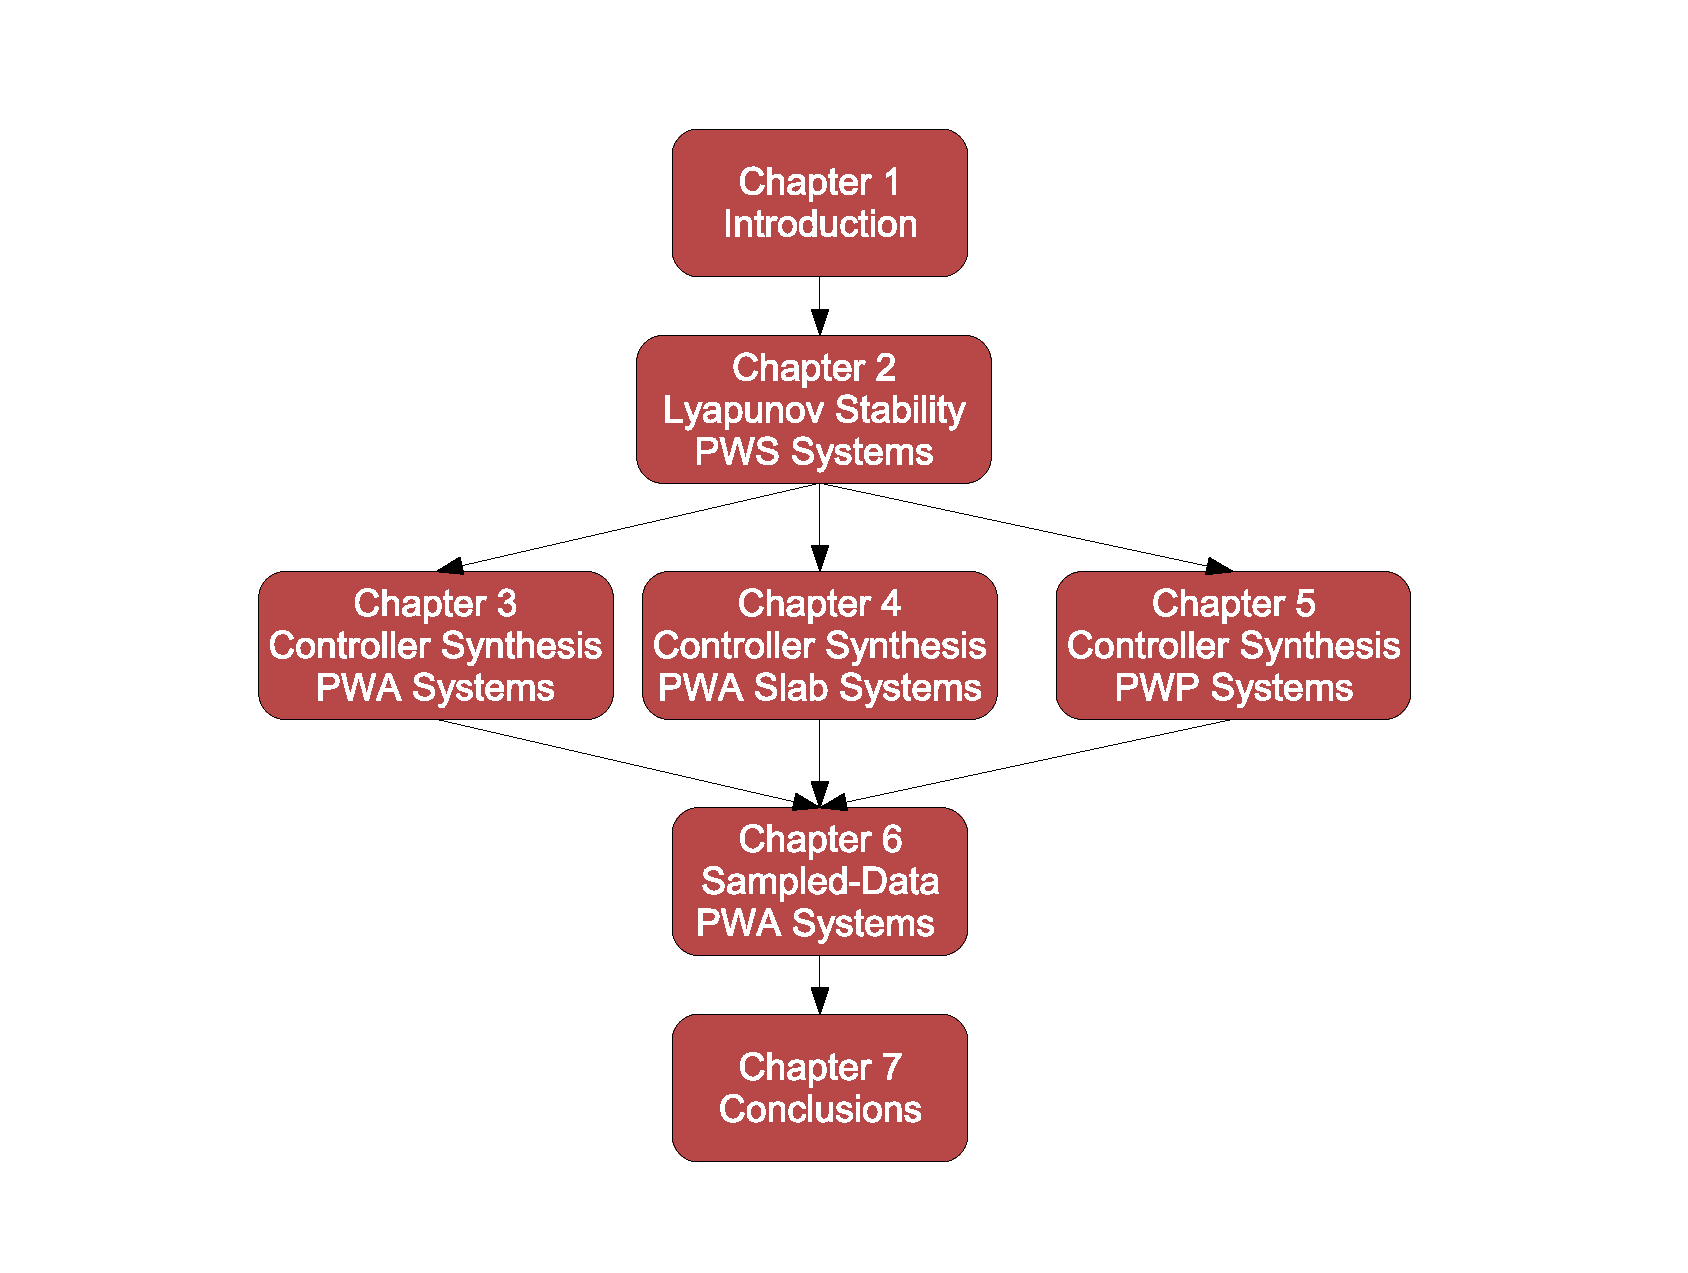
\includegraphics{images/CrossOutline.eps}}}
  }

  \section{Introduction}
  \frame
  {
    \frametitle{Introduction}

    \centerline{\scalebox{0.36}{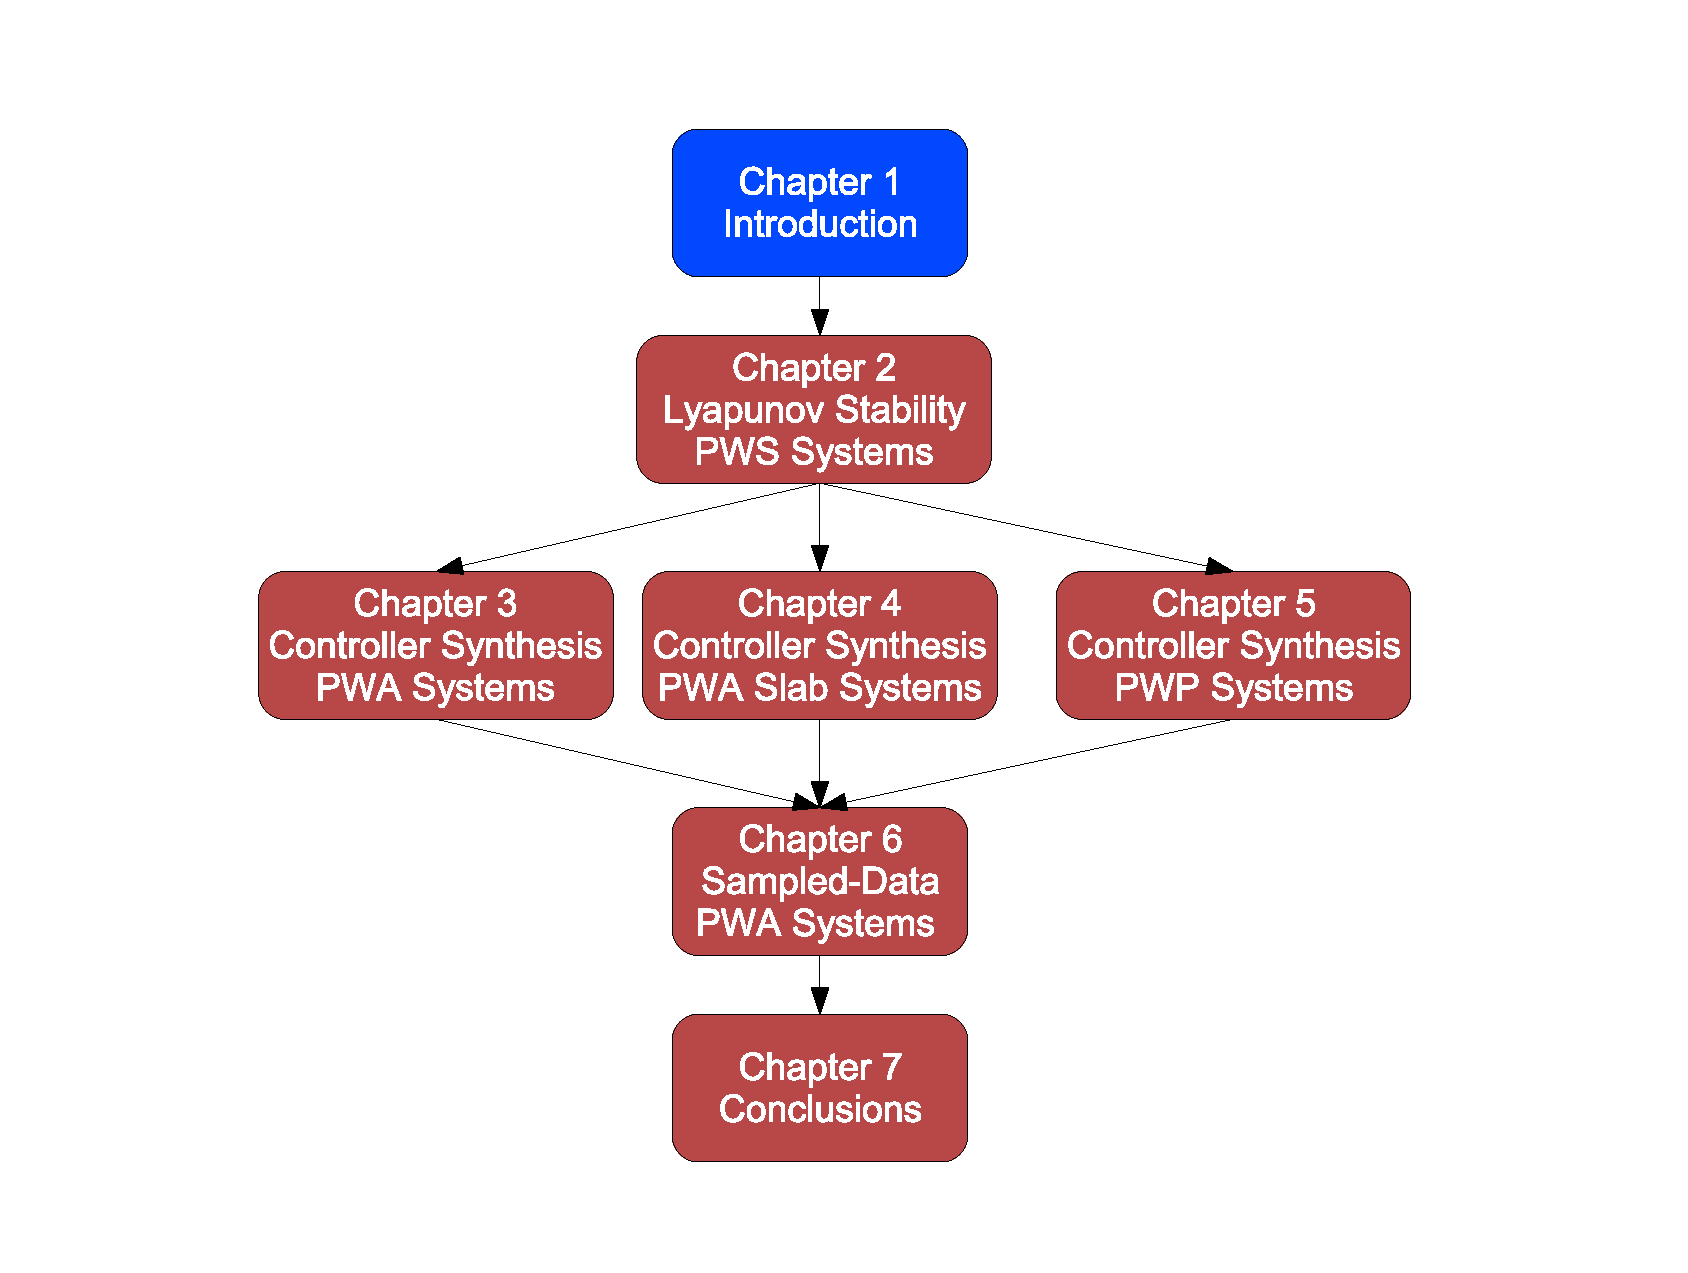
\includegraphics{images/Cross1.eps}}}
  }
    \frame
  {
  \frametitle{Practical Motivation}
    \centerline{\scalebox{0.17}{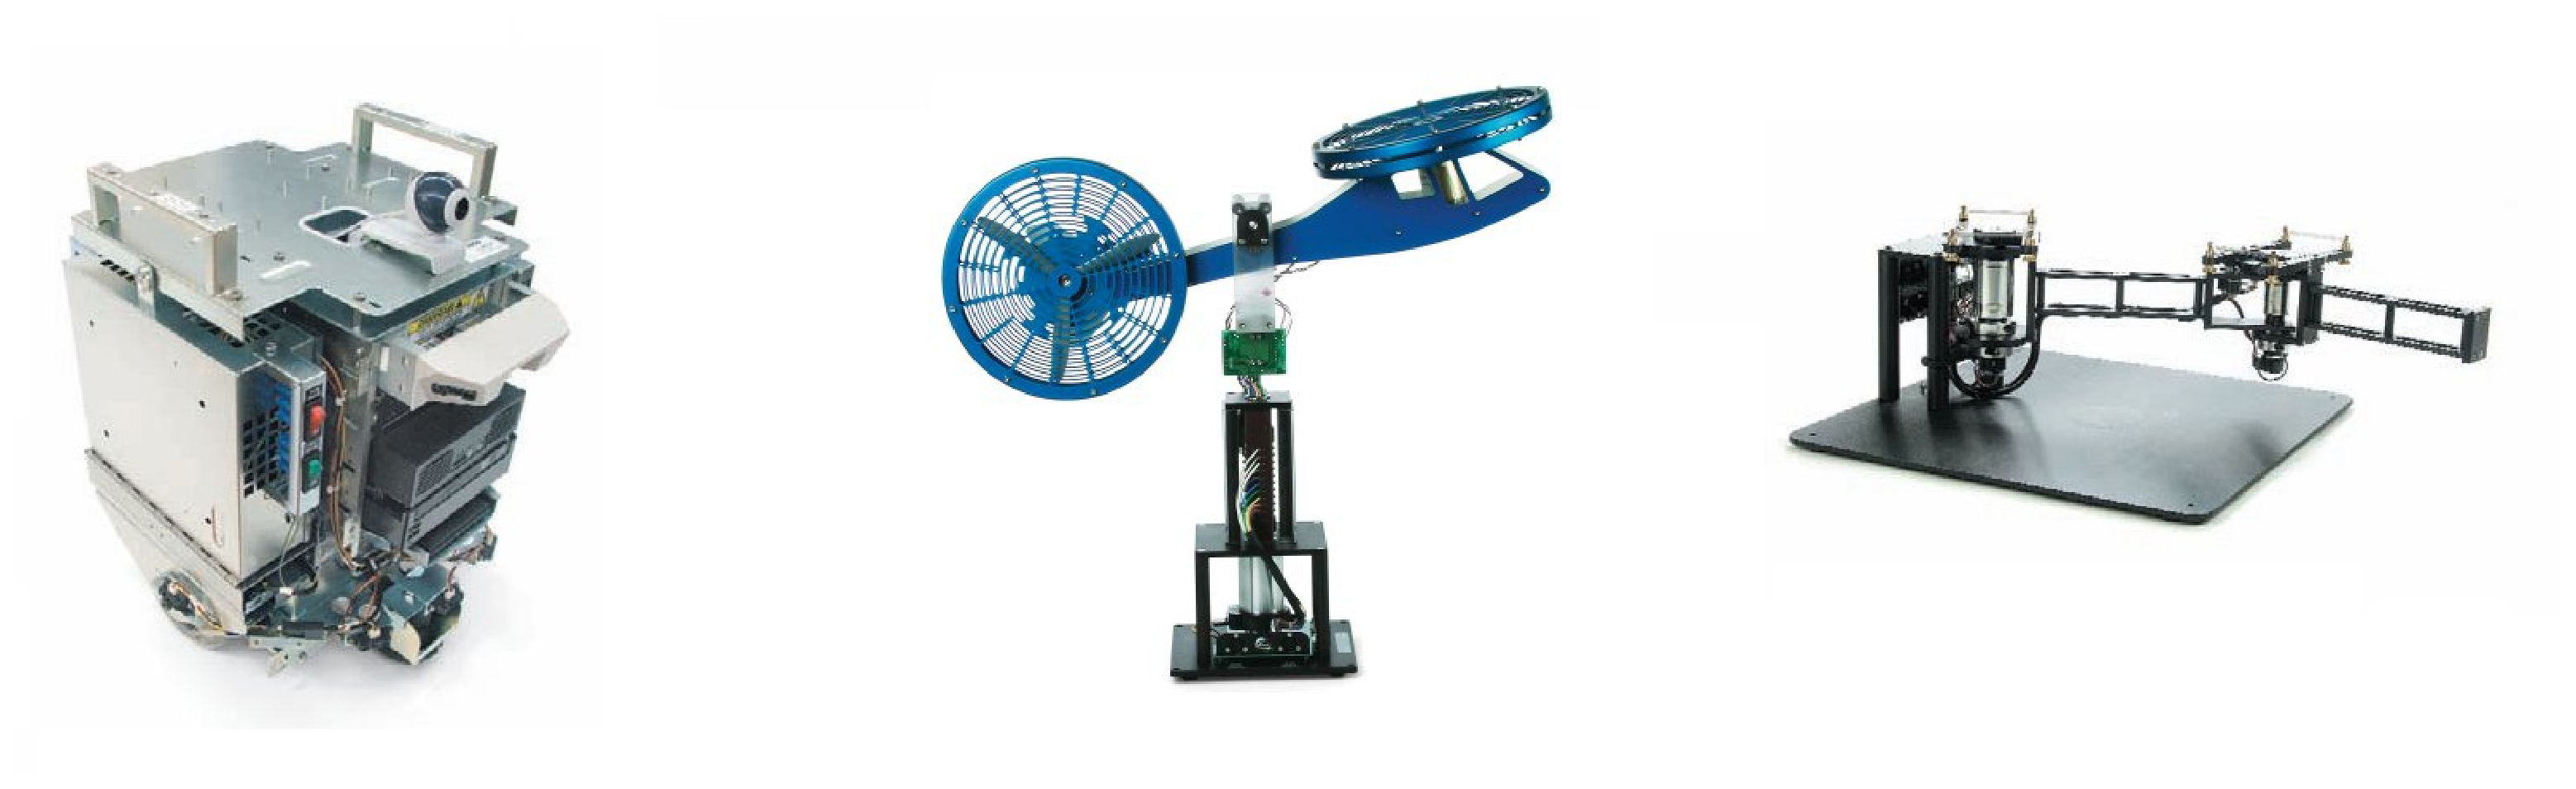
\includegraphics{images/QuanserMHF.eps}}}  
    {\scriptsize \copyright Quanser}
    \centerline{\scalebox{0.7}{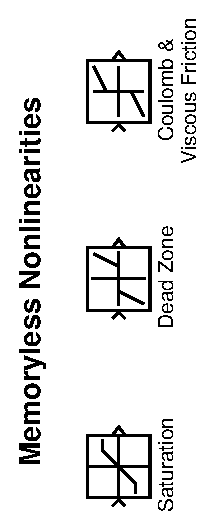
\includegraphics[angle=-90]{images/MLNL.eps}}}
}
    \frame[shrink=4]
  {
  \frametitle{Theoretical Motivation}
  \begin{itemize}
  \item {\scriptsize \href{http://www.cds.caltech.edu/~murray/archive/topten/}{\emph{Richard Murray, California Institute of Technology: ``}}} 
  \begin{center}
  \begin{tabular}{|c|p{9cm}|}
\hline
\textbf{Rank} &	\textbf{Top Ten Research Problems in Nonlinear Control}\\\hline
{\scriptsize 10} &	{\scriptsize Building representative experiments for evaluating controllers} \\\hline
{\scriptsize 9} &	{\scriptsize Convincing industry to invest in new nonlinear methodologies} \\\hline
{\scriptsize 8} &	{\scriptsize Recognizing the difference between regulation and tracking}\\\hline
{\scriptsize \textbf{{\blue 7}}} &	{\scriptsize \textbf{{\blue Exploiting special structure to analyze and design controllers}}}\\\hline
{\scriptsize\textbf{{\blue 6}}} &	{\scriptsize \textbf{{\blue Integrating good linear techniques into nonlinear methodologies}}}\\\hline
{\scriptsize 5} &	{\scriptsize Recognizing the difference between performance and operability}\\\hline
{\scriptsize 4} &	{\scriptsize Finding nonlinear normal systems for control}\\\hline
{\scriptsize\textbf{{\blue 3}}} &	{\scriptsize\textbf{{\blue Global robust stabilization and local robust performance}}}\\\hline
{\scriptsize 2} &	{\scriptsize Magnitude and rate saturation}\\\hline
{\scriptsize\textbf{{\blue 1}}} &	{\scriptsize\textbf{{\blue Writing numerical software for implementing nonlinear theory}}}\\\hline
  \end{tabular}
  \end{center}
  \item \parbox{10cm}{{\scriptsize ...This is more or less a way for me to think online, so I wouldn't take any of this too seriously.''}}
  \end{itemize}
}

  \frame
  {
    \frametitle{Special Structure}
		\begin{itemize}
		\item Piecewise smooth system: 
		\beq
		\dot x=f(x)+g(x)u 
		\eeq  
		where $f(x)$ and $g(x)$ are piecewise continuous and bounded functions of $x$. 
		\end{itemize}
		     \centerline{\scalebox{0.3}{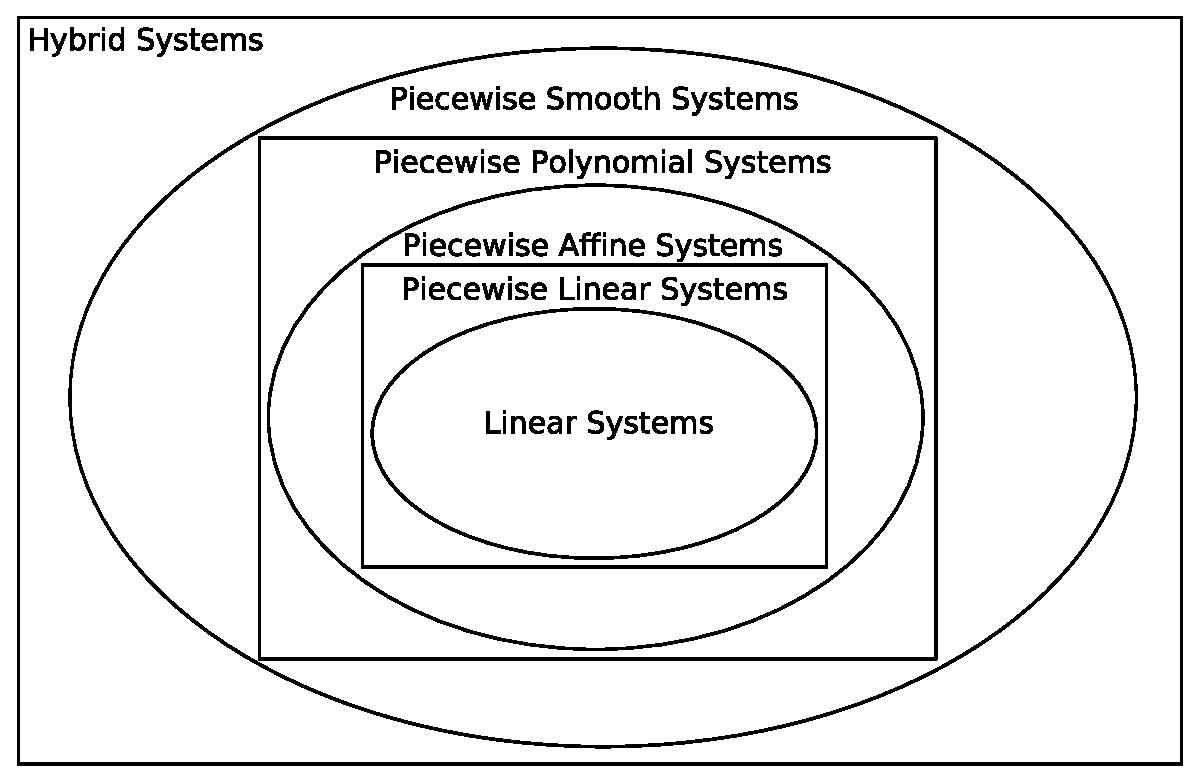
\includegraphics{images/pwssystem.eps}}}
}
  \frame
  {
    \frametitle{Objective}
    To develop a \textbf{computational tool} to design controllers for \textbf{piecewise smooth systems} using \textbf{convex optimization} techniques.
    \begin{itemize}
    \item<2-> Why convex optimization? 
    \begin{itemize}
    \item There are numerically efficient tools to solve convex optimization problems.
    \item Linear Matrix Inequalities ({\green LMI})
    \item Sum of Squares ({\green SOS}) programming
    \end{itemize}
    \end{itemize}
  }

  \frame
  {
    \frametitle{Literature}
    \begin{itemize}
    \item Hassibi and Boyd (1998) - Quadratic stabilization and control of piecewise linear systems - {\red Limited to piecewise linear controllers} for PWA slab systems
    \item Johansson and Rantzer (2000) - Piecewise linear quadratic optimal control - {\red No guarantee for stability}
    \item Feng (2002) - Controller design and analysis of uncertain piecewise linear systems - {\red All local subsystems should be stable}
    \item Rodrigues and How (2003) - Observer-based control of piecewise affine systems - {\red Bilinear matrix inequality}
    \item Rodrigues and Boyd (2005) - Piecewise affine state feedback for piecewise affine slab systems using convex optimization -  Stability analysis and synthesis using {\red parametrized linear matrix inequalities}
%    \item Rodrigues and Boukas (2006) - Piecewise linear H$_\infty$ controller synthesis with application to inventory control of switched production systems - L$_2$ gain synthesis for piecewise linear systems 
    \end{itemize}
}

  \frame
  {
    \frametitle{Major Contributions}
\begin{enumerate}
\item To propose a two-step controller synthesis method for a class of uncertain nonlinear systems described by PWA differential inclusions.
\item To introduce for the first time a duality-based interpretation of PWA systems. This enables controller synthesis for PWA slab systems to be formulated as a convex optimization problem. 
\item To propose a nonsmooth backstepping controller synthesis for PWP systems. 
\item To propose a time-delay approach to stability analysis of sampled-data PWA systems.
\end{enumerate}
}

  \section[Chapter 2]{Lyapunov Stability}
  \frame
  {
    \frametitle{Lyapunov Stability for Piecewise Smooth Systems}

    \centerline{\scalebox{0.36}{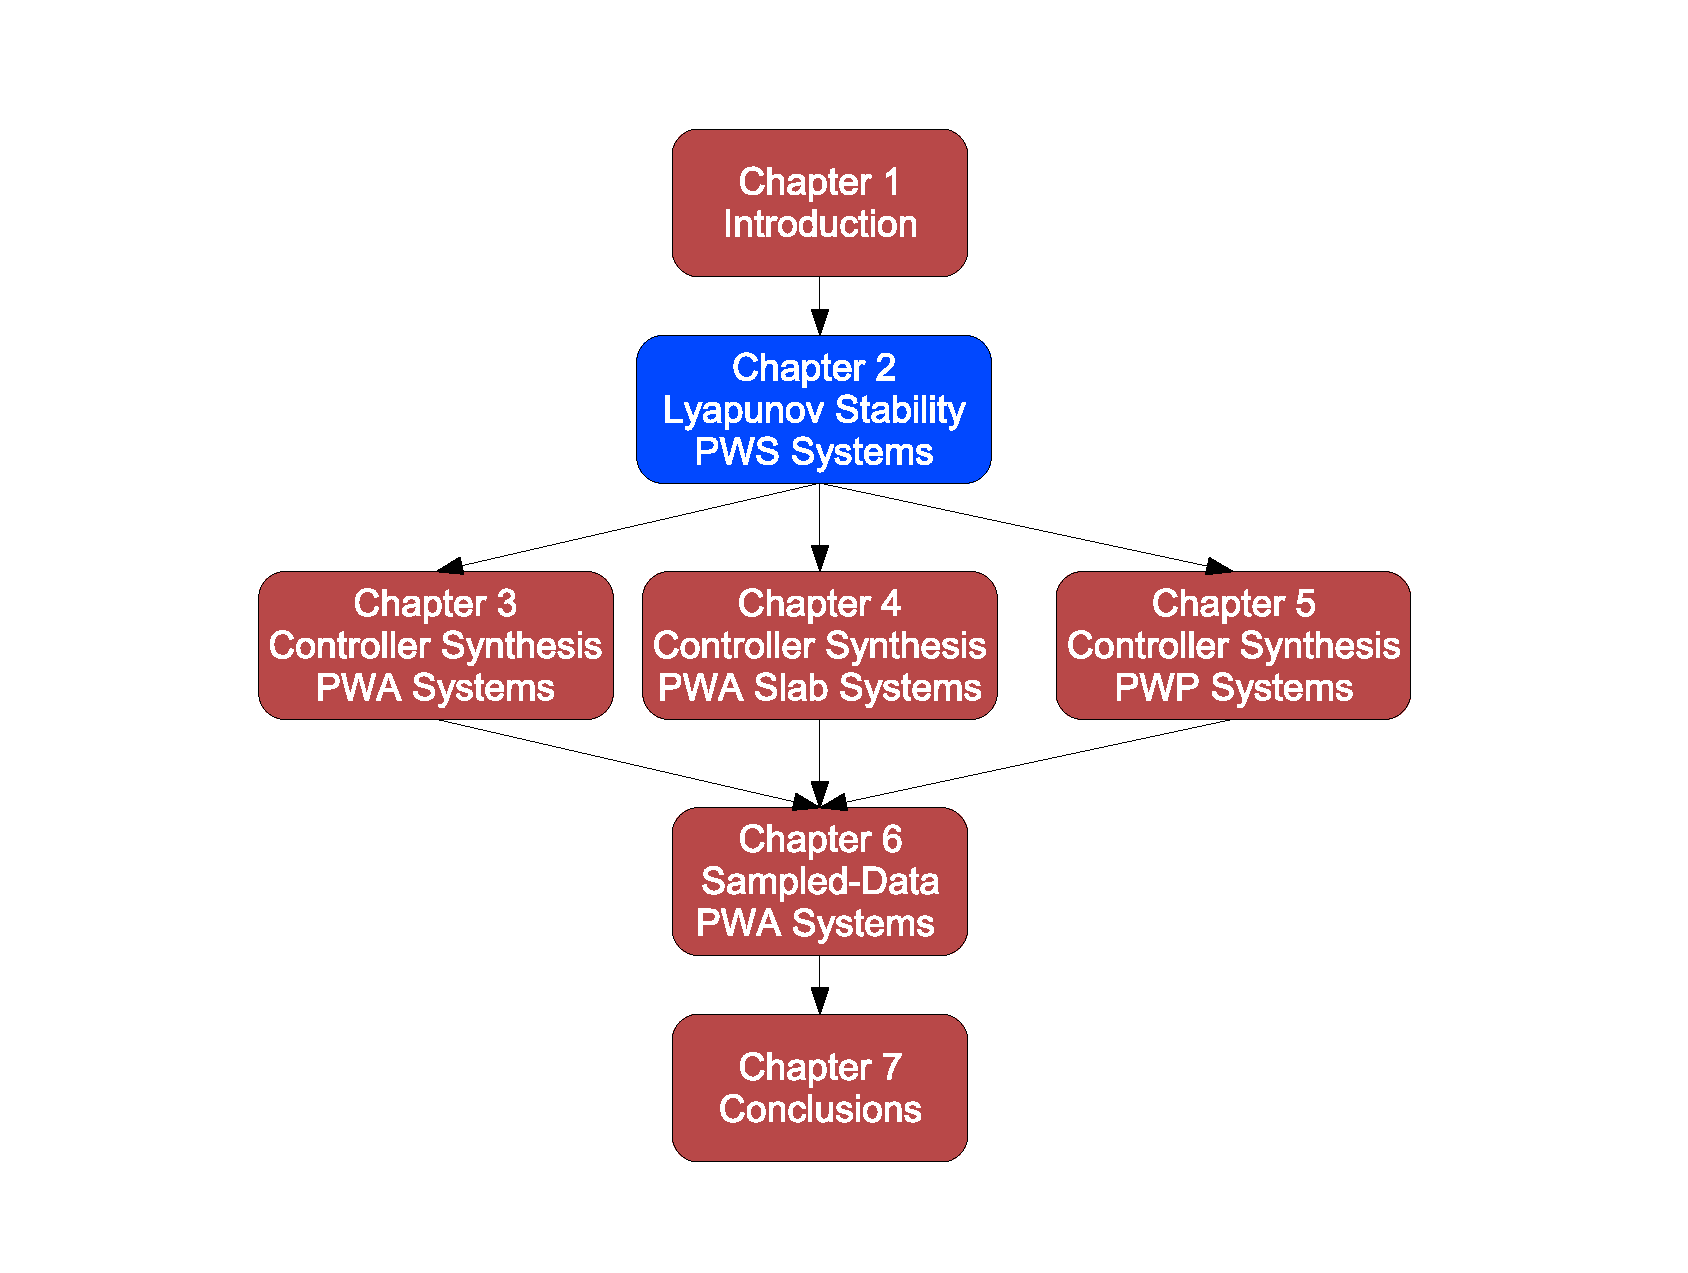
\includegraphics{images/Cross2.eps}}}
  }
  
  \frame[shrink=6]
  {
    \frametitle{Lyapunov Stability for Piecewise Smooth Systems}
    \begin{center}
    \begin{theorem}[2.1]
    For nonlinear system $\dot x(t)=f(x(t))$, if there exists a continuous function $V(x)$ such that
\begin{eqnarray*}
&&V(x^\star)=0\\
&&V(x)>0 \text{ for all }x\neq x^\star\text{ in }{\cal X}\\
&& t_1\leq t_2\Rightarrow V(x(t_1))\geq V(x(t_2))
\end{eqnarray*}
then $x=x^\star$ is a stable equilibrium point. Moreover if there exists a continuous function $W(x)$ such that
\begin{eqnarray*}
&&W(x^\star)=0\\
&&W(x)>0 \text{ for all }x\neq x^\star\text{ in }{\cal X}\\
&& t_1\leq t_2\Rightarrow V(x(t_1))\geq V(x(t_2))+\int_{t_1}^{t_2}W(x(\tau))d\tau
\end{eqnarray*}
and 
\beq
\|x\|\rightarrow\infty\Rightarrow V(x)\rightarrow\infty 
\eeq
then all trajectories in ${\cal X}$ asymptotically converge to $x=x^\star$.
    \end{theorem}
    \end{center}
}
  \frame
  {
    \frametitle{Lyapunov Stability for Piecewise Smooth Systems}
    Why nonsmooth analysis?
\begin{itemize}
\item Discontinuous vector fields
\item Piecewise smooth Lyapunov functions
\end{itemize}
    \begin{center}
    \begin{tabular}{|l|c|c|}
    \hline
    \multirow{2}{*}{\textbf{Lyapunov Function}} & \multicolumn{2}{|c|}{\textbf{Vector Field}}\\\cline{2-3}
      &Continuous &Discontinuous \\\hline
    Smooth  & {\Large {\green \faIcon[regular]{smile}}} & {\Large {\green \faIcon[regular]{smile}}}\\\hline
    Piecewise Smooth& {\Large {\green \faIcon[regular]{smile}}} & {\Large{\red \faIcon[regular]{frown}}} \\\hline
    \end{tabular}
    \end{center}
}

  \section[Chapter 3]{Extension of linear controllers to PWA controllers}

  \frame
  {
    \frametitle{Extension of local linear controllers to global PWA controllers for uncertain nonlinear systems}

    \centerline{\scalebox{0.36}{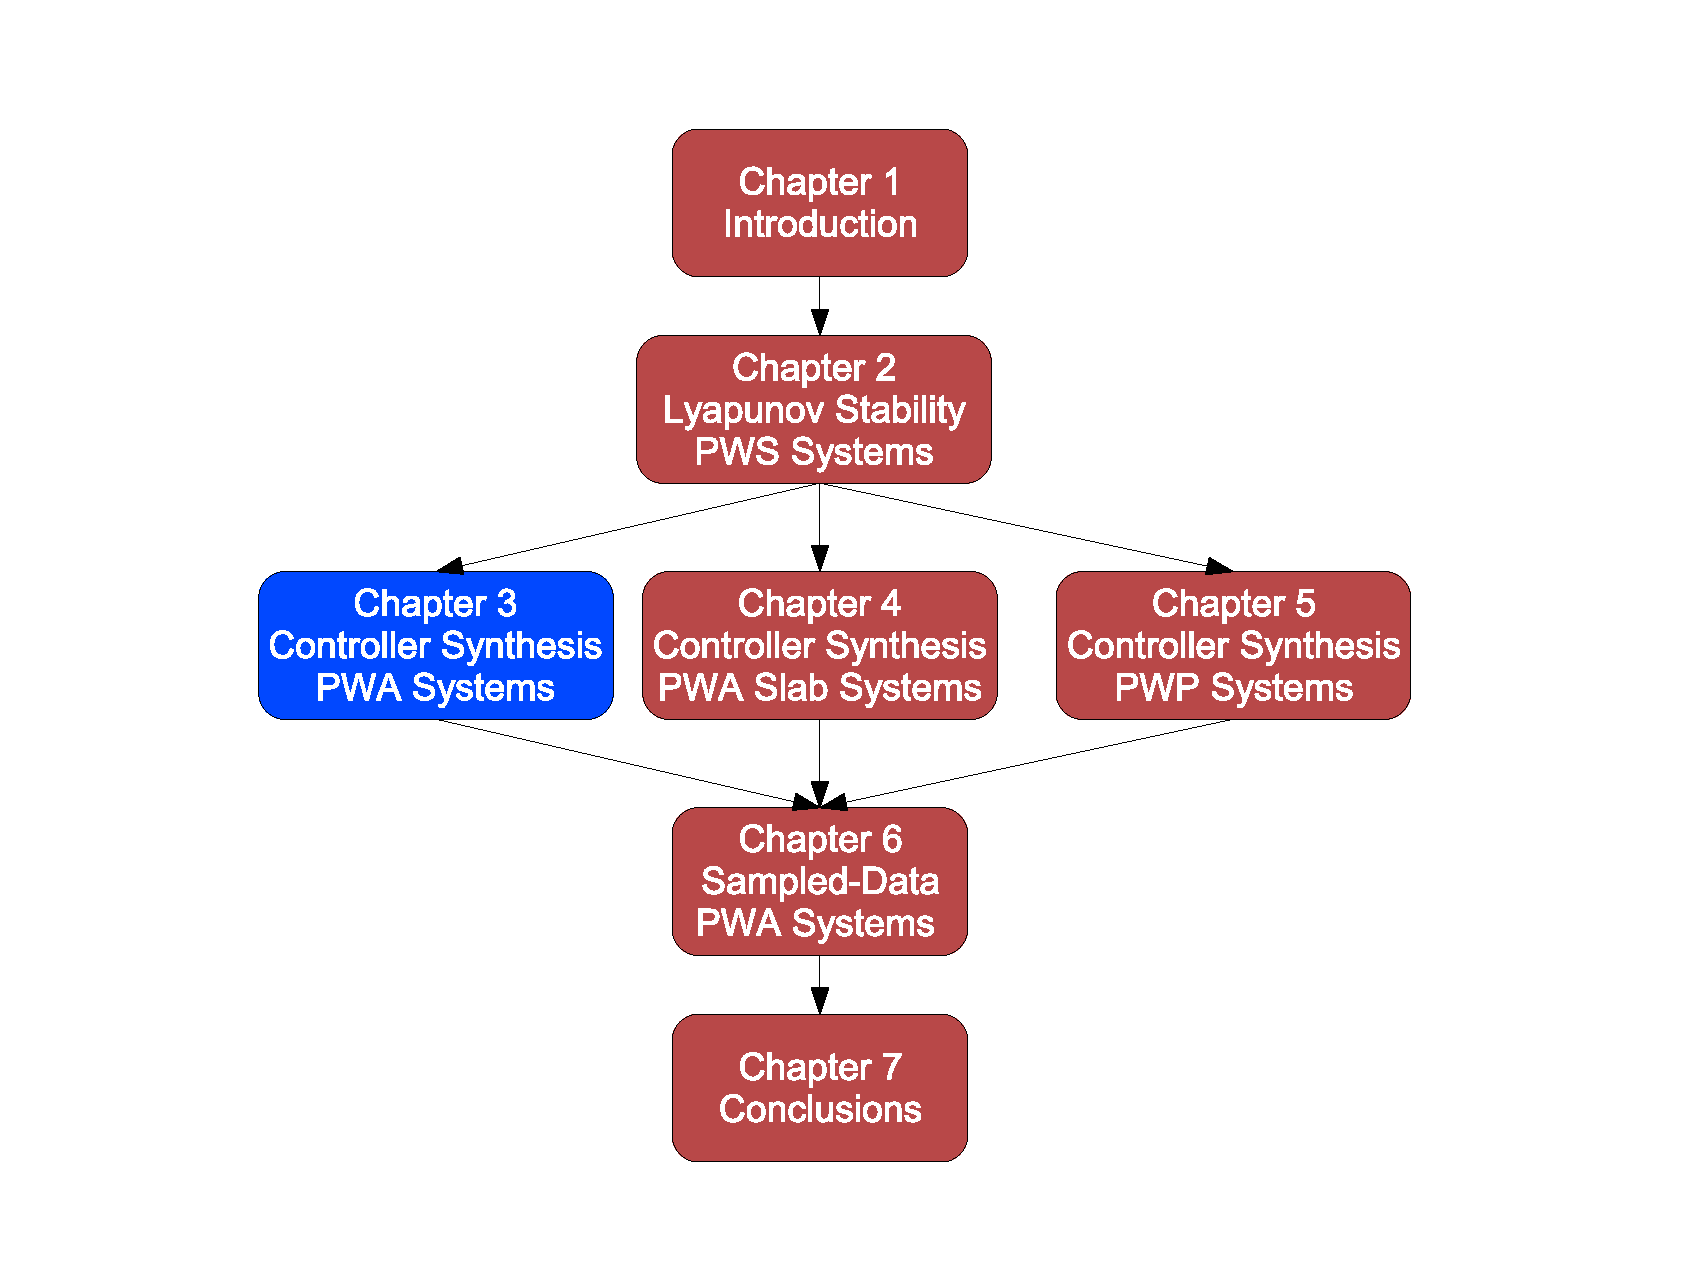
\includegraphics{images/Cross3.eps}}}
  }

  \frame
  {
    \frametitle{Extension of linear controllers to PWA controllers}
    Objectives:
    \begin{itemize}
\item \textbf{Global robust stabilization} and \textbf{local robust performance}
\item Integrating good \textbf{linear techniques} into \textbf{nonlinear methodologies}
\end{itemize}
  }

  \frame
  {
    \frametitle{PWA Differential Inclusions}
    \begin{itemize}
    \item Consider the following \textbf{uncertain} nonlinear system
\beq
\dot x=f(x)+g(x)u
\eeq
Let 
\beq
\dot x\in\CO\{\sigma_{1}(x,u),\ldots,\sigma_\KA(x,u)\}
\eeq
where
\beq
\sigma_\kappa(x,u)=A_{i\kappa}x+a_{i\kappa}+B_{i\kappa} u, x\in\overline\RR_i,
\eeq
with  
\beq
\RR_i = \{ x| E_ix+e_i \succ 0\}, \text{ for } i=1,\ldots,M
\eeq
$\succ$ represents an elementwise inequality.
\end{itemize}
  }

  \frame
  {
    \frametitle{PWA Differential Inclusions}
\centerline{PWA bounding envelope for a nonlinear function}  
\centerline{\resizebox{8cm}{!}{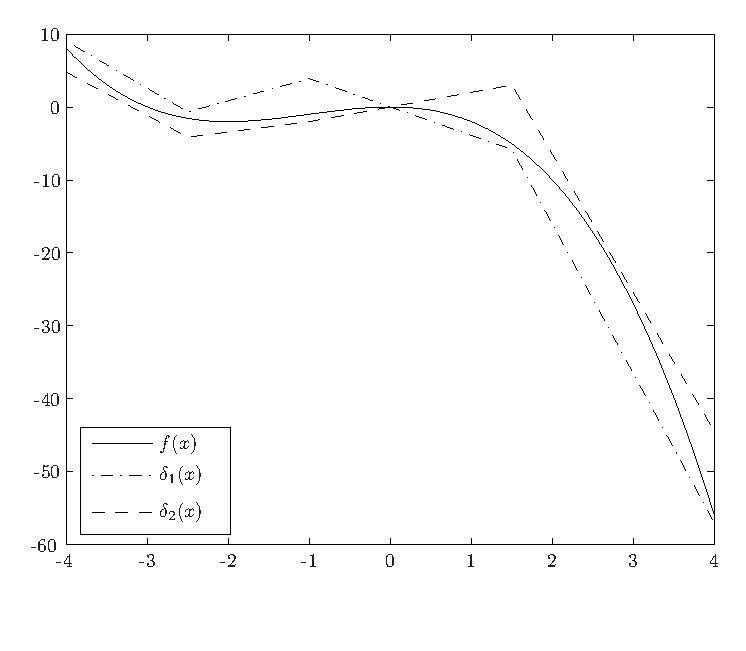
\includegraphics{images/BndEnv.pdf}}}
}

  \frame
  {
    \frametitle{Extension of linear controllers to PWA controllers}
    \centerline{\scalebox{0.36}{\includegraphics{images/Lin2PWA.eps}}}
  }

  \frame
  {
    \frametitle{Extension of linear controllers to PWA controllers}
\begin{theorem}[3.2]
Let there exist matrices $\bar P_i=\bar P_i^T$, $\bar K_i$, $Z_i$, $\bar Z_i$, $\Lambda_{i\kappa}$ and $\bar \Lambda_{i\kappa}$ that verify the conditions for all $i=1,\ldots,M$, $\kappa=1,\ldots,\KA$ and for a given decay rate $\alpha>0$, desired equilibrium point $x^\star$, linear controller gain $\bar K_{i^\star}$ and $\epsilon>0$, then \textbf{all trajectories of the nonlinear system} in $\cal X$ asymptotically converge to $x=x^\star$.
\end{theorem}
\begin{itemize}
\item<2-> If the conditions are feasible, the resulting PWA controller provides global robust stability and local robust performance.
\item<3-> The synthesis problem includes a set of Bilinear Matrix Inequalities (BMI). In general, it is not convex.
\end{itemize}
}  
 
  \section[Chapter 4]{Controller synthesis for PWA slab differential inclusions}
  \frame
  {
    \frametitle{Controller synthesis for PWA slab differential inclusions: a duality-based convex optimization approach}
    \centerline{\scalebox{0.36}{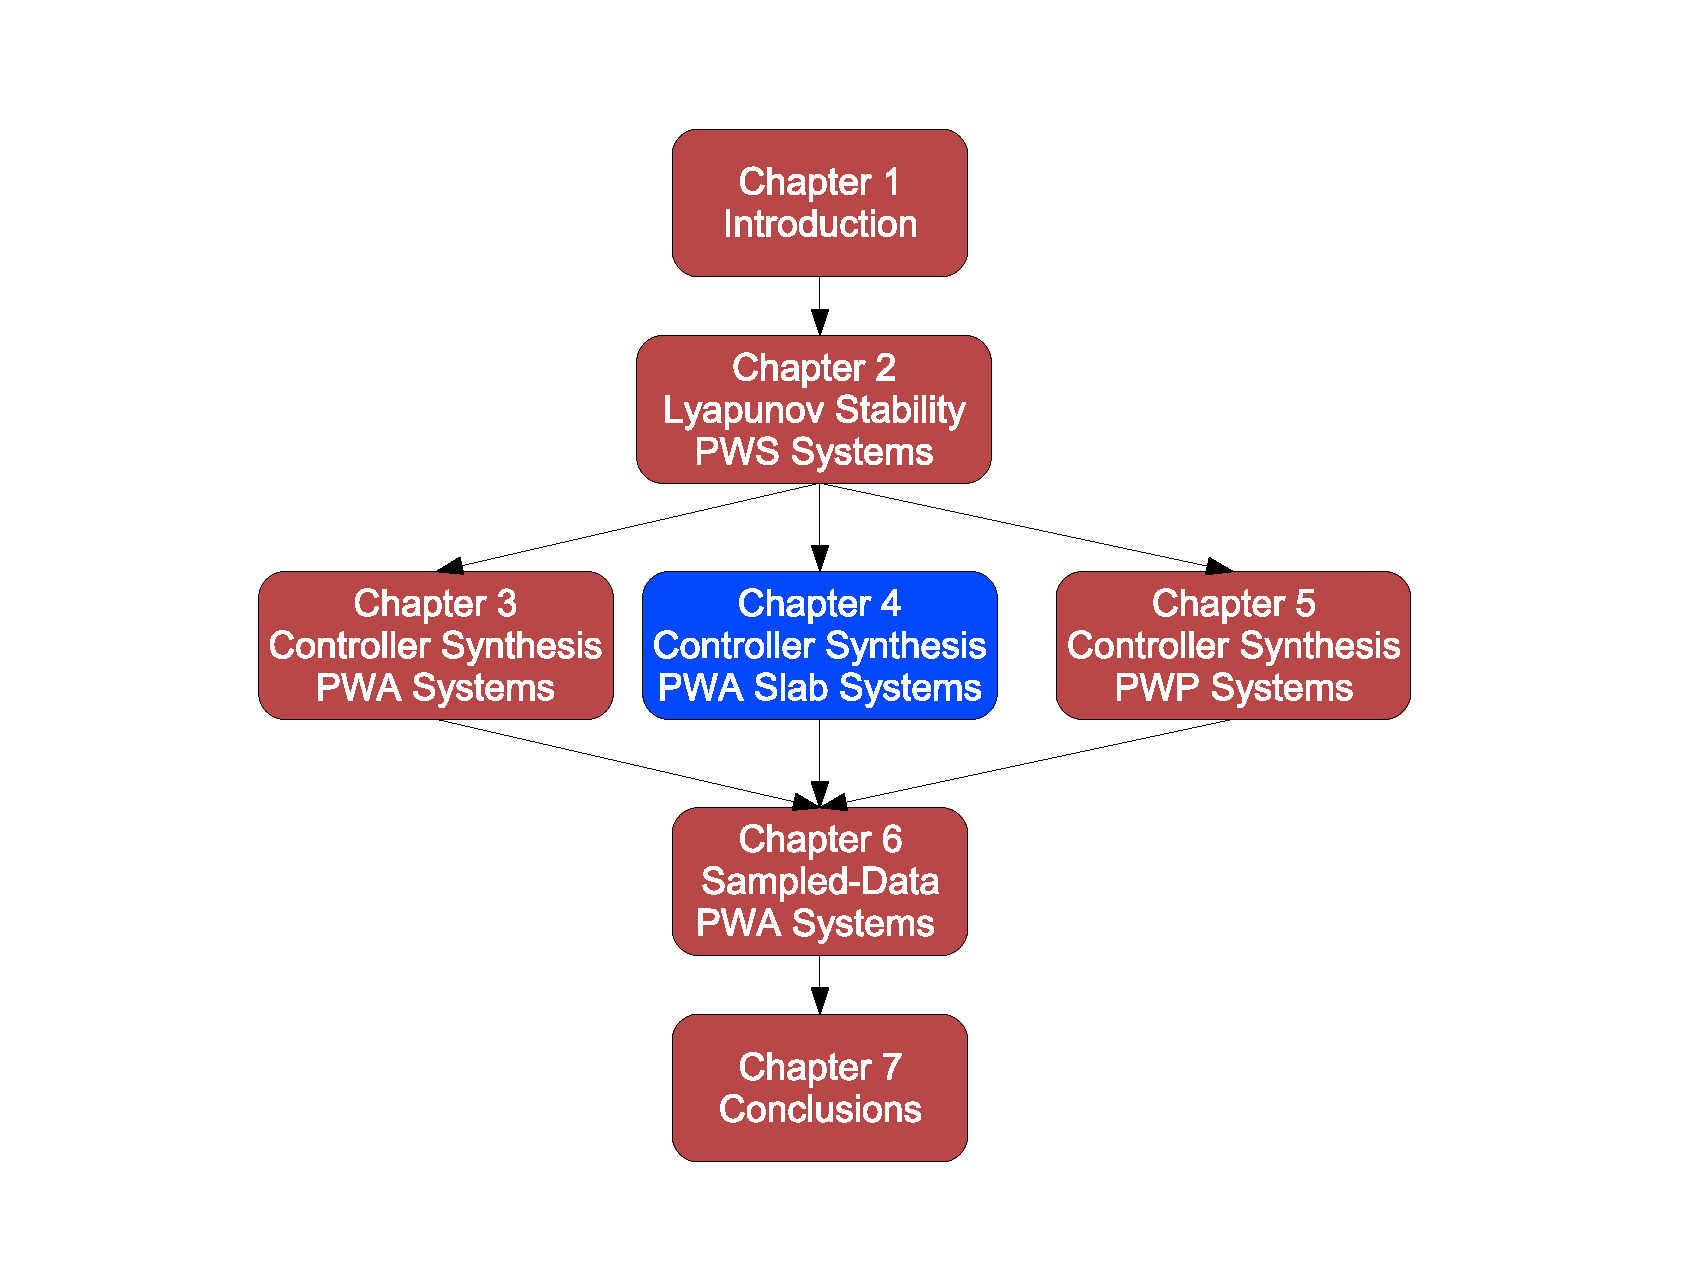
\includegraphics{images/Cross4.eps}}}
  }

  \frame
  {
    \frametitle{Controller synthesis for PWA slab differential inclusions: a duality-based convex optimization approach}
    {\Large Objective:}
    \begin{itemize}
    \item To formulate controller synthesis for \textbf{stability} and \textbf{L$_2$ gain performance} of piecewise affine \textbf{slab} differential inclusions as a set of {\green LMI}s.
    \end{itemize}
}  

\frame[shrink=5]
  {
    \frametitle{L$_2$ Gain Analysis for PWA Slab Differential Inclusions}
    \begin{itemize}
    \item PWA slab differential inclusion:
\begin{align}
\dot x \in& {\red \CO}\{A_{i\kappa}x+a_{i\kappa}+B_{w_{i\kappa}}w, \kappa=1,2 \},\ 
(x,w)\in{\red {\mathcal R}_i^{{\cal X}\times{\cal W}}}\nonumber\\
y \in & {\red \CO}\{C_{i\kappa}x+{\red c_{i\kappa}}+D_{w_{i\kappa}}w, \kappa=1,2 \}\nonumber\\
{\red \RR_i^{{\cal X}\times{\cal W}}}=&\{(x,w) |\ \|L_ix+l_i+{\red M_i}w\|<1\}\nonumber
\end{align}
\item {\red Parameter set}:
\beq
\Phi =\left\{ \left.\bmat{ccc}A_{i\kappa_1}&a_{i\kappa_1}&B_{w_{i\kappa_1}}\\L_i&l_i&M_i\\C_{i\kappa_2}&c_{i\kappa_2}&D_{w_{i\kappa_2}}\ \emat\right|\ i=1,\ldots,M,\ \kappa_1=1,2,\ \kappa_2=1,2\right\}
\eeq
\end{itemize}
}
  
\frame
  {
\frametitle{A duality-based convex optimization approach}
\centerline{{\Large {\red Dual Parameter Set}}}
\beq
\Phi^\TR =\left\{\left.\bmat{ccc}A_{i\kappa_1}^\TR&L_i^\TR&C_{i\kappa_2}^\TR\\a_{i\kappa_1}^\TR&l_i&c_{i\kappa_2}^\TR\\B_{w_{i\kappa_1}}^\TR&M_i^\TR&D_{w_{i\kappa_2}}^\TR\emat\ \right|i=1,\ldots,M,\ \kappa_1=1,2,\ \kappa_2=1,2\right\}
\eeq  
}   

\frame{
    \frametitle{LMI Conditions for L$_2$ Gain Analysis}
\centerline{\Large {\red Parameter Set}}
\centerline{$P>0$,}
\beq
	\bmat{cc} A^\TR_{i\kappa_1}P+PA_{i\kappa_1}+C_{i\kappa_2}^TC_{i\kappa_2}&*\\
	B_{w_{i\kappa_1}}^\TR P+D_{w_{i\kappa_2}}^\TR C_{i\kappa_2}&-\gamma^2I+D_{w_{i\kappa_2}}^\TR D_{w_{i\kappa_2}}
	\emat< 0
\eeq
for $i\in{\mathcal I}(0,0)$, $\kappa_1=1,2$ and $\kappa_2=1,2$ and  
$\lambda_{i\kappa_1\kappa_2}<0$
{\scriptsize
\beq
	\bmat{ccc}\bmatp{c} A^\TR_{i\kappa_1}P+PA_{i\kappa_1}\\+C_{i\kappa_2}^TC_{i\kappa_2}\\+\lambda_{i\kappa_1\kappa_2}L_{i}^TL_{i}\ematp&*&*\\[2mm]	a_{i\kappa_1}^TP+c_{i\kappa_2}^TC_{i\kappa_2}+\lambda_{i\kappa_1\kappa_2}l_{i}L_{i}&\lambda_{i\kappa_1\kappa_2}(l_{i}^2-1)+c_{i\kappa_2}^Tc_{i\kappa_2}&*\\[2mm]
\bmatp{c}B_{w_{i\kappa_1}}^\TR P\\+D_{w_{i\kappa_2}}^\TR C_{i\kappa_2}\\+\lambda_{i\kappa_1\kappa_2}M_i^\TR L_i\ematp&D_{w_{i\kappa_2}}^\TR c_{i\kappa_2}+\lambda_{i\kappa_1\kappa_2}l_iM_i^\TR &\bmatp{c}-\gamma^2I\\+D_{w_{i\kappa_2}}^\TR D_{w_{i\kappa_2}}\\+\lambda_{i\kappa_1\kappa_2}M_i^\TR M_i\ematp
	\emat< 0
\eeq
for $i\notin{\mathcal I}(0,0)$, $\kappa_1=1,2$ and $\kappa_2=1,2$
}
}

\frame{
    \frametitle{LMI Conditions for L$_2$ Gain Analysis}
\centerline{\Large {\red Dual Parameter Set}}
\centerline{$Q>0$,}
\beq
	\bmat{cc} A_{i\kappa_1}Q+QA^\TR_{i\kappa_1}+B_{w_{i\kappa_1}} B_{w_{i\kappa_1}}^\TR&*\\
C_{i\kappa_2}Q+D_{w_{i\kappa_2}}B_{w_{i\kappa_1}}^\TR&-\gamma^2I+D_{w_{i\kappa_2}}D_{w_{i\kappa_2}}^\TR
	\emat< 0
\eeq
for $i\in{\mathcal I}(0,0)$, $\kappa_1=1,2$ and $\kappa_2=1,2$ and 
$\mu_{i\kappa_1\kappa_2}<0$
{\scriptsize
\beq
	\bmat{ccc} \bmatp{c}A_{i\kappa_1}Q+QA^\TR_{i\kappa_1}\\+B_{w_{i\kappa_1}} B_{w_{i\kappa_1}}^\TR\\+\mu_{i\kappa_1\kappa_2}a_{i\kappa_1}a_{i\kappa_1}^\TR\ematp&*&*\\	L_iQ+M_iB_{w_{i\kappa_1}}^\TR+\mu_{i\kappa_1\kappa_2}l_{i}a_{i\kappa_1}^\TR&\mu_{i\kappa_1\kappa_2}(l_{i}^2-1)+M_iM_i^\TR&*\\	\bmatp{c}C_{i\kappa_2}Q+D_{w_{i\kappa_2}}B_{w_{i\kappa_1}}^\TR\\+\mu_{i\kappa_1\kappa_2}c_{i\kappa_2}a_{i\kappa_1}^\TR\ematp&D_{w_{i\kappa_2}}M_i^\TR+\mu_{i\kappa_1\kappa_2}l_{i}c_{i\kappa_2}&\bmatp{c}-\gamma^2I\\+D_{w_{i\kappa_2}}D_{w_{i\kappa_2}}^\TR\\+\mu_{i\kappa_1\kappa_2}c_{i\kappa_2}c_{i\kappa_2}^\TR\ematp	\emat< 0
\eeq
 for $i\notin{\mathcal I}(0,0)$, $\kappa_1=1,2$ and $\kappa_2=1,2$
}
}  


\frame{
    \frametitle{PWA L$_2$ gain controller synthesis}
\begin{itemize}
\item The goal is to limit the L$_2$ gain from $w$ to $y$ using the following PWA controller:
\beq
u=K_ix+{\red k_i},\ x\in{\mathcal R}_i
\eeq
\item New variables:
\begin{eqnarray*}
Y_i&=&K_i Q\\
Z_i&=&\mu_i k_i\\
W_i&=&\mu_i k_i k_i^\TR
\end{eqnarray*}
\item{\red Problem}: $W_i$ is not a linear function of the unknown parameters $\mu_i$, $Y_i$ and $Z_i$.
\end{itemize}
}

\frame{
\frametitle{A duality-based convex optimization approach}
Proposed solutions:
\begin{itemize}
\item<1-> \emph{Convex relaxation}: Since $W_i=\mu_i k_i k_i^\TR\leq0$, if the synthesis inequalities are satisfied with $W_i=0$, they are satisfied with any $W_i\leq0$. Therefore, the synthesis problem can be made convex by omitting $W_i$.  
\item<2-> \emph{Rank minimization}: Note that $W_i=\mu_i k_i k_i^\TR\leq0$ is the solution of the following rank minimization problem:
\beq
\begin{array}{l}
\min \RK X_i\\
\text{s.t. }X_i=\bmat{cc}W_i&Z_i\\Z_i^\TR &\mu_i\emat\leq 0
\end{array}
\eeq
Rank minimization is also not a convex problem. However, trace minimization works practically well as a heuristic solution
\beq
\min \TC X_i,  \text{ s.t. }X_i=\bmat{cc}W_i&Z_i\\Z_i^\TR &\mu_i\emat\leq 0
\eeq
\end{itemize}
}

\frame
  {
    \frametitle{A duality-based convex optimization approach}
    The following problems for PWA slab differential inclusions with PWA outputs were formulated as a set of {\green LMI}s:
    \begin{itemize}
    \item Stability analysis (Propositions 4.1 and 4.2)      
    \item L$_2$ gain analysis (Propositions 4.3 and 4.4) 
    \item Stabilization using PWA controllers (Propositions 4.5 and 4.6)
    \item PWA L$_2$ gain controller synthesis (Propositions 4.7 and 4.8)
    \end{itemize}
}  
  
\section[Chapter 5]{Backstepping Controller Synthesis for PWP Systems}

  \frame
  {
    \frametitle{Backstepping Controller Synthesis for PWP Systems: A Sum of Squares Approach}
    \centerline{\scalebox{0.36}{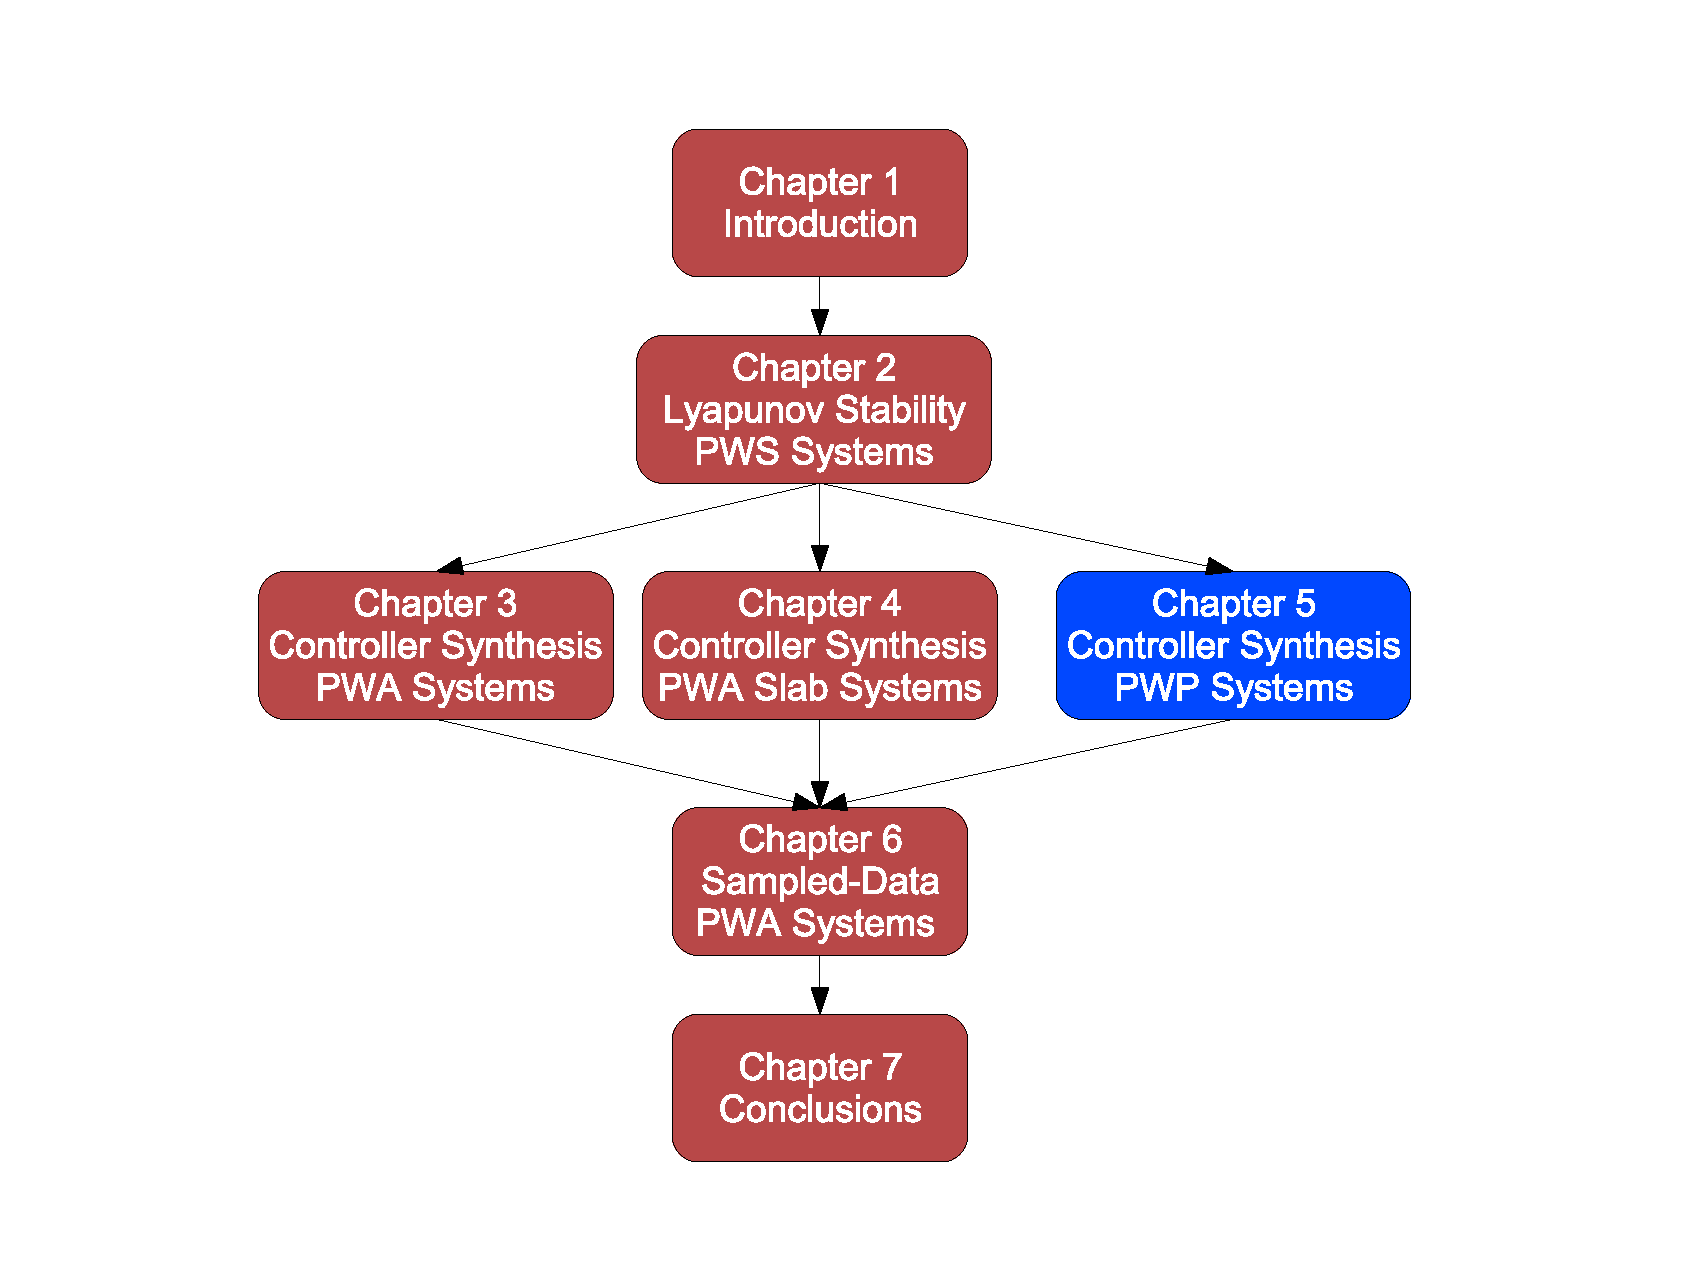
\includegraphics{images/Cross5.eps}}}
  }

  \frame
  {
    \frametitle{Backstepping Controller Synthesis for PWP Systems: A Sum of Squares Approach}
    
    Objective:
    \begin{itemize}
    \item<1-> To formulate controller synthesis for a class of piecewise polynomial systems as a {\green Sum of Squares (SOS)} programming.
\item<2-> SOSTOOLS, a MATLAB toolbox that handles the general SOS programming, was developed by S. Prajna, A. Papachristodoulou and P. Parrilo. 
    \beq
		p(x) = \sum_{i=1}^m f_i^2(x) \geq 0
		\eeq
\end{itemize}
}


\frame[shrink=4]
  {
    \frametitle{Backstepping Controller Synthesis for PWP Systems: A Sum of Squares Approach}

\begin{itemize}
    \item PWP system in \emph{strict feedback from} 
\beq
\left\{\begin{array}{ll}
\dot x_1=f_{1i_1}(x_1)+g_{1i_1}(x_1)x_2,&\text{ for } x_1\in\PR_{1i_1}\\
\dot x_2=f_{2i_2}(x_1,x_2)+g_{2i_2}(x_1,x_2)x_3,&\text{ for } \bmat{c}x_1\\x_2\emat\in\PR_{2i_2} \\
\vdots&\\
\dot x_k=f_{ki_k}(x_1,x_2,\ldots,x_k)+g_{ki_k}(x_1,x_2,\ldots,x_k)u,&\text{ for } \bmat{c}x_1\\x_2\\\vdots\\x_k\emat\in\PR_{ki_k}\\
\end{array}\right.
\eeq
where
\beq
\PR_{ji_j} = \left\{\left.\bmat{c}x_1\\\vdots\\x_j\emat \right| E_{ji_j}(x_1,\ldots,x_j)\succ0 \right\}
\eeq
\end{itemize}
}

  \frame
  {
    \frametitle{Sampled-Data PWA Systems: A Time-Delay Approach}
Motivation: Toycopter, a 2 DOF helicopter model

    \centerline{\scalebox{0.36}{\includegraphics{images/QuanserHelicopterPic.eps}}}
  }

\frame
  {  
    \frametitle{Sampled-Data PWA Systems: A Time-Delay Approach}
    Example: 
    \begin{itemize}
    \item<1->Pitch model of the experimental helicopter:
\begin{align*}
\dot x_1 =& x2\\
\dot x_2 =& \frac{1}{I_{yy}}(-m_{heli}l_{cgx}g\cos(x_1)-m_{heli}l_{cgz}g\sin(x_1)-F_{kM}\sign(x_2)\\
&-F_{vM}x_2+u)
\end{align*} 
where $x_1$ is the pitch angle and $x_2$ is the pitch rate.
\item Nonlinear part:
\beq
f(x_1) = -m_{heli}l_{cgx}g\cos(x_1)-m_{heli}l_{cgz}g\sin(x_1)
\eeq
\item PWA part:
\beq
f(x_2) = -F_{kM}\sign(x_2)
\eeq
\end{itemize}
}

\frame
  {  
    \frametitle{Sampled-Data PWA Systems: A Time-Delay Approach}
\centerline{\resizebox{8cm}{!}{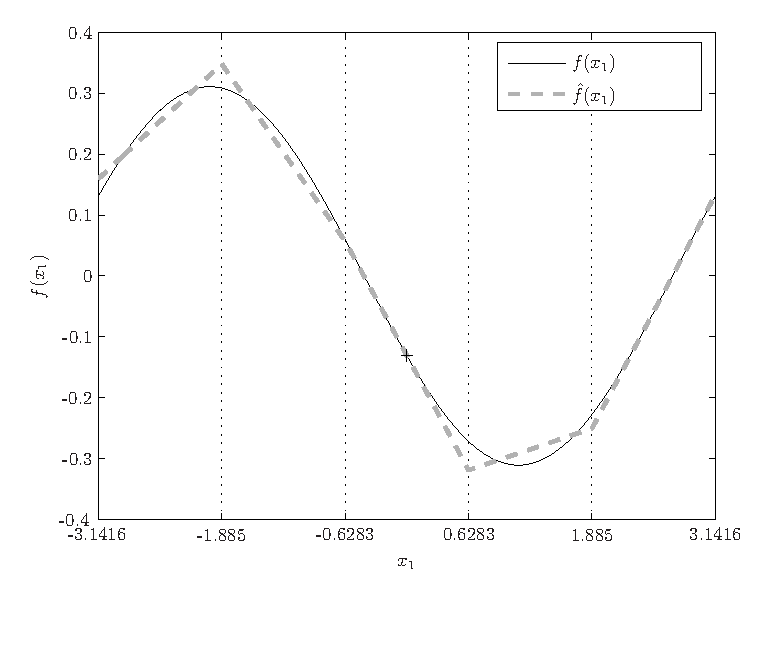
\includegraphics{images/SDHelExPWA.pdf}}}
\centerline{PWA approximation - Helicopter model}
}

\frame
  {  
  \frametitle{Sampled-Data PWA Systems: A Time-Delay Approach}
\centerline{\resizebox{8cm}{!}{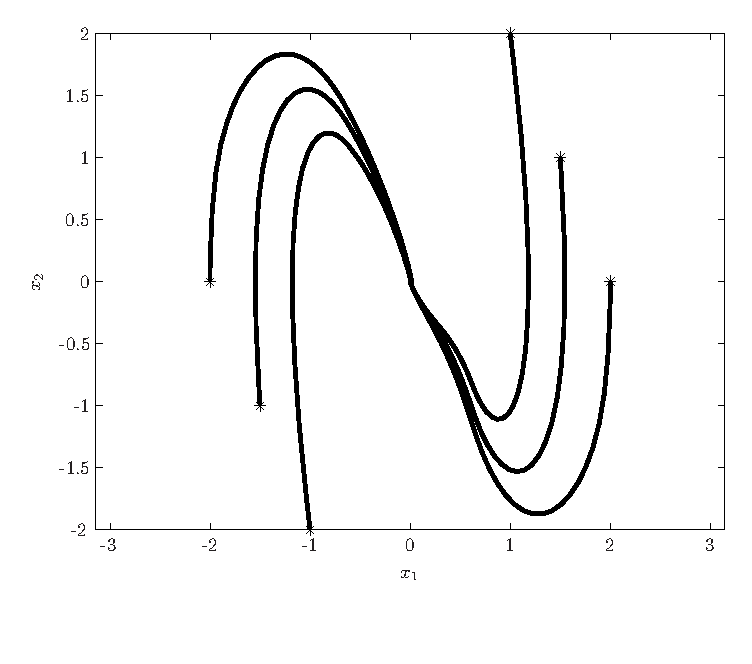
\includegraphics{images/ConHeli.pdf}}}
\centerline{Continuous time PWA controller}    
}

\section[Chapter 6]{Sampled-Data PWA Systems}

  \frame
  {
    \frametitle{Sampled-Data PWA Systems: A Time-Delay Approach}

    \centerline{\scalebox{0.36}{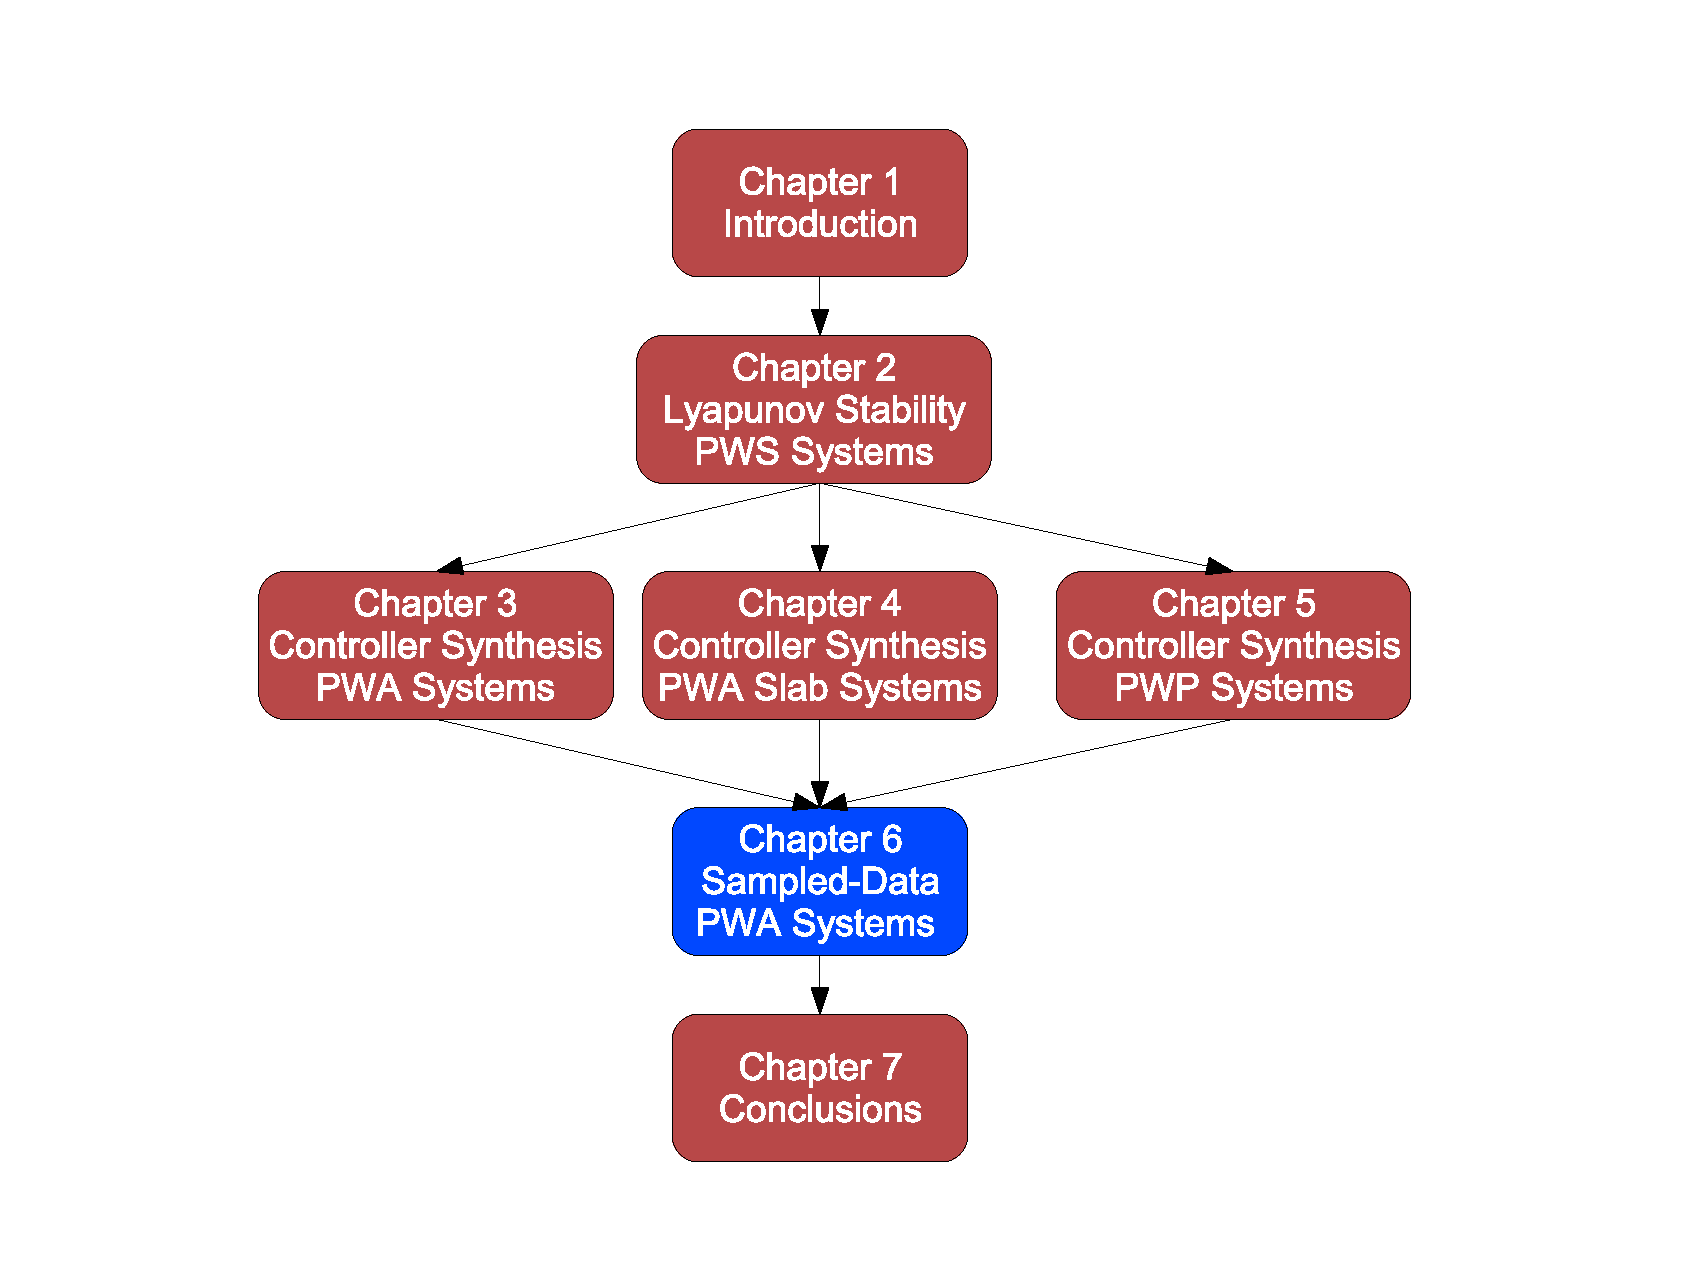
\includegraphics{images/Cross6.eps}}}
  }

  \frame
  {
    \frametitle{Sampled-Data PWA Systems: A Time-Delay Approach}
\begin{itemize}
\item Sampled-data PWA controller
\beq
u(t)=K_ix(t_k)+k_i,\ x(t_k)\in\RR_i
\eeq
\centerline{\scalebox{0.5}{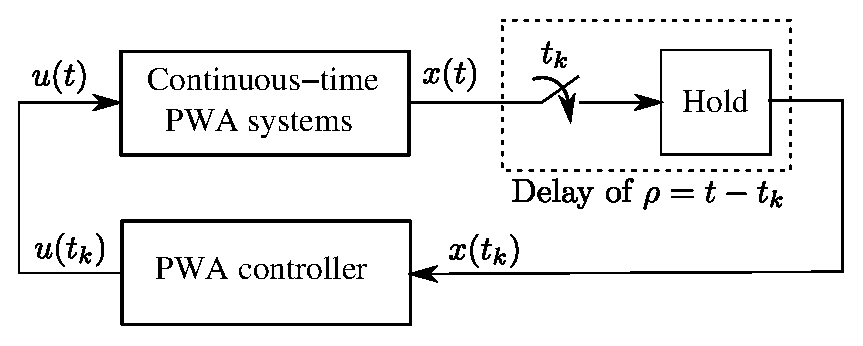
\includegraphics{images/SDPWA.eps}}}
\end{itemize}
  }

  \frame
  {
    \frametitle{Sampled-Data PWA Systems: A Time-Delay Approach}
\begin{itemize}
\item The closed-loop system can be rewritten as
\beq
\dot x(t)=A_ix(t)+a_i+B_i(K_ix(t_k)+k_i)+B_iw,
\eeq
for $x(t)\in\RR_i$ and $x(t_k)\in\RR_j$ where
\beq
w(t) = (K_j-K_i)x(t_k)+(k_j-k_i),\ x(t)\in\RR_i,\ x(t_k)\in\RR_j
\eeq
The input $w(t)$ is a result of the fact that $x(t)$ and $x(t_k)$ are not necessarily in the same region. 
\end{itemize}
}

  \frame
  {
    \frametitle{Sampled-Data PWA Systems: A Time-Delay Approach}
\begin{theorem}[6.1]
For the sampled-data PWA system, assume there exist symmetric positive matrices $P,R,X$ and matrices $N_i$ for $i=1,\ldots,M$ such that the conditions are satisfied and let there be constants $\Delta_K$ and $\Delta_k$ such that
\beq
\|w\|\leq \Delta_K\|x(t_k)\|+\Delta_k
\eeq
Then, all the trajectories of the sampled-data PWA system  in ${\cal X}$ converge to the following invariant set
\beq
\Omega = \{x_s|\ V(x_s,\rho)\leq \sigma_a\mu_\theta^2+\sigma_b \}
\eeq
\end{theorem}
}

\frame
  {  
    \frametitle{Sampled-Data PWA Systems: A Time-Delay Approach}
Solving an optimization problem to maximize $\tau_M$ subject to the constraints of the main theorem and $\eta>\gamma>1$ leads to
\beq
{\green \tau_M^\star = 0.2193 }
\eeq
}

\frame
  {  
  \frametitle{Sampled-Data PWA Systems: A Time-Delay Approach}
\centerline{\resizebox{8cm}{!}{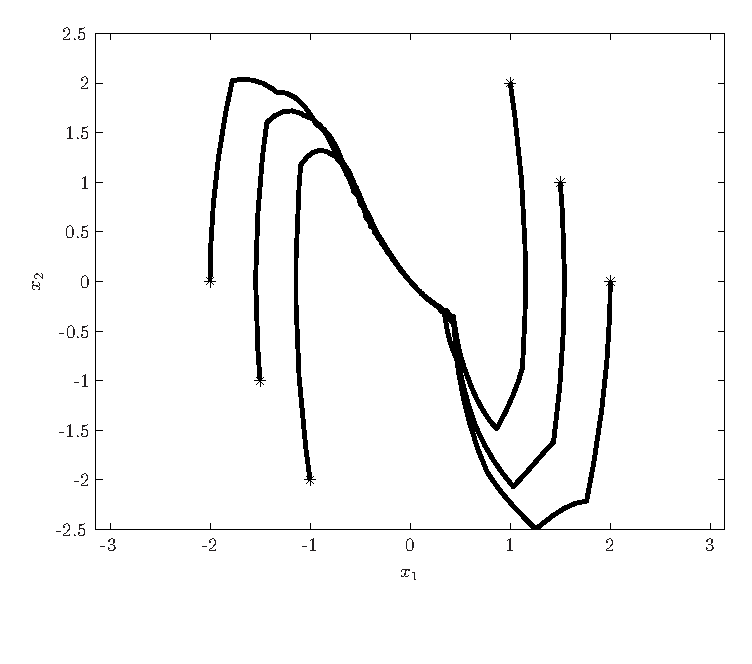
\includegraphics{images/SDHeli.pdf}}}
\centerline{Sampled data PWA controller for $T_s=0.2193$}    
}

\frame
  {  
  \frametitle{Sampled-Data PWA Systems: A Time-Delay Approach}
\centerline{\resizebox{8cm}{!}{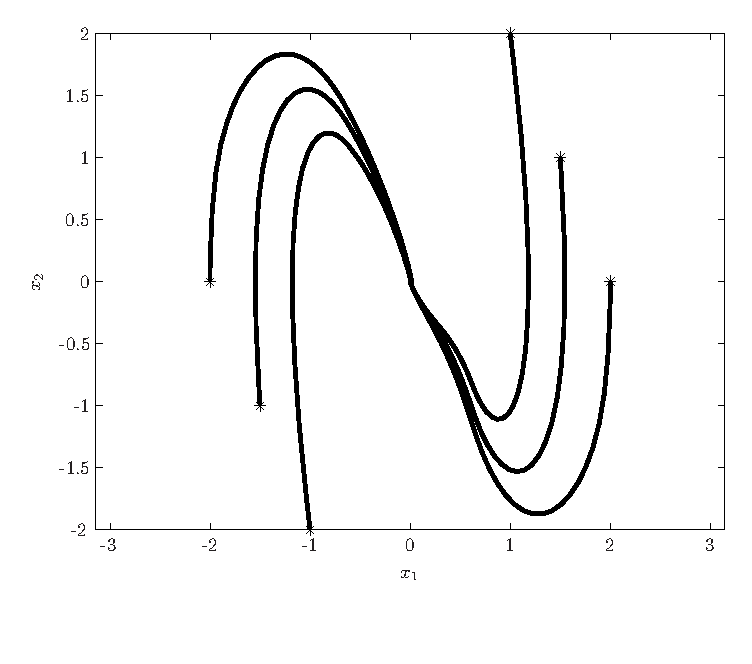
\includegraphics{images/ConHeli.pdf}}}
\centerline{Continuous time PWA controller}    
}

\frame
{
  \frametitle{Breaking News}
\begin{itemize}
\item<1-> The day before yesterday, I almost had a heart attack when...
\item<2-> I found a {\Large {\red LITTLE MINUS SIGN MISTAKE}} in the proof of Theorem 6.1.
\item<3-> {\green Good news} is that fixing the mistake slightly changes the LMI conditions for PWA systems and that does not affect the numerical results much. For example for the helicopter model, $\tau_M$ was $0.2193$. Now, it is $0.2175$.
\item<4-> {\red Bad news} is that for linear systems I get exactly the LMI conditions of [82]. Therefore, the result for linear systems and the linear example are no longer valid.
\item<5-> {\green Good news} is that I can still keep my friendship with my undergrad classmate who is the first author of [82]. 
\end{itemize}
}

\section{Conclusions}

  \frame
  {
    \frametitle{Conclusions}

    \centerline{\scalebox{0.36}{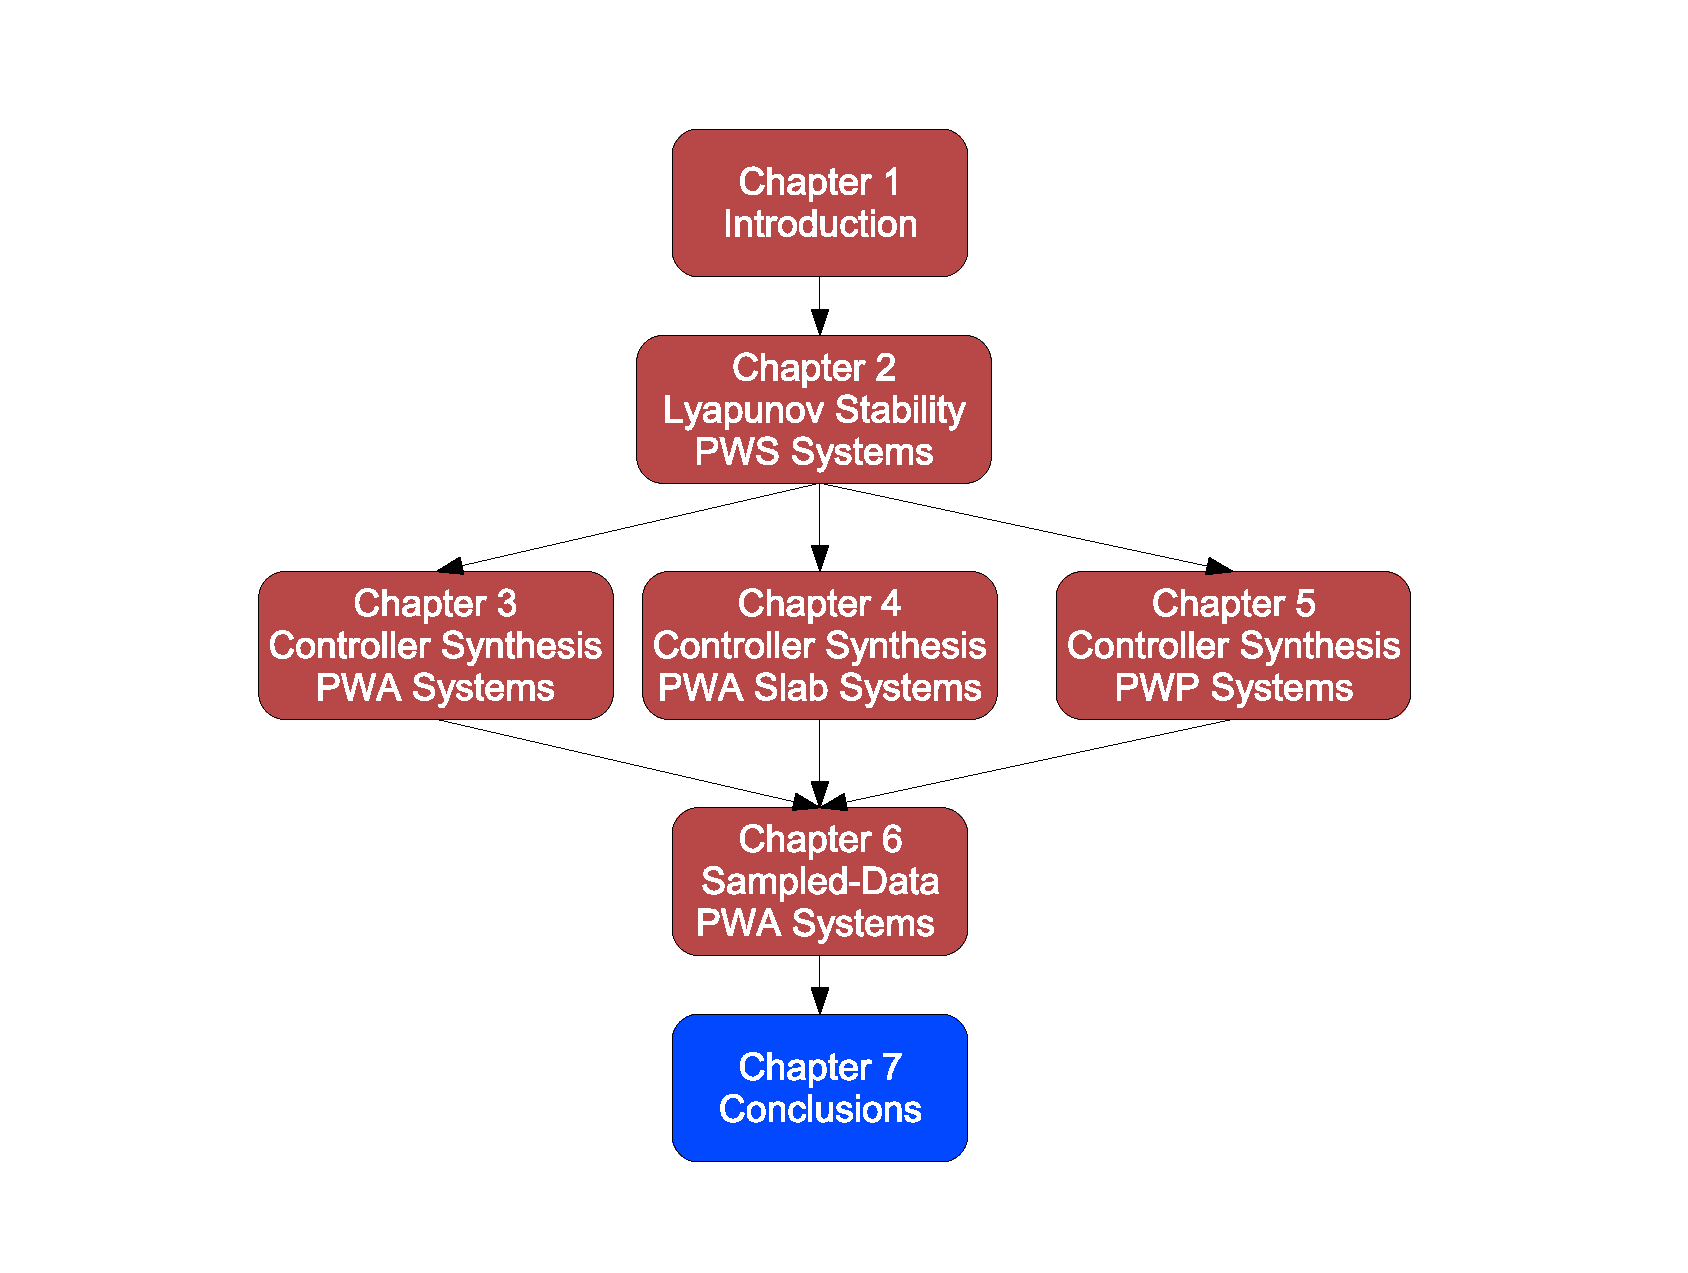
\includegraphics{images/Cross7.eps}}}
  }

  \frame
  {
    \frametitle{Summary of Major Contributions}
\begin{enumerate}
\item To propose a two-step controller synthesis method for a class of uncertain nonlinear systems described by PWA differential inclusions.
\item To introduce for the first time a duality-based interpretation of PWA systems. This enables controller synthesis for PWA slab systems to be formulated as a convex optimization problem. 
\item To propose a nonsmooth backstepping controller synthesis for PWP systems. 
\item To propose a time-delay approach to stability analysis of sampled-data PWA systems.
\end{enumerate}
}
  \frame
  {
    \frametitle{Publications}

\begin{enumerate}
\item  B. Samadi and L. Rodrigues, ``Extension of local linear controllers to global piecewise affine controllers for uncertain nonlinear systems,'' accepted for publication in the \emph{International Journal of Systems Science}.
\item  B. Samadi and L. Rodrigues, ``Controller synthesis for piecewise affine slab differential inclusions: a duality-based convex optimization approach,'' under second revision for publication in \emph{Automatica}.
\item B. Samadi and L. Rodrigues, ``Backstepping Controller Synthesis for Piecewise Polynomial Systems: A Sum of Squares Approach,'' in preparation
\item B. Samadi and L. Rodrigues, ``Sampled-Data Piecewise Affine Systems: A Time-Delay Approach,'' to be submitted.
\end{enumerate} 
}

  \frame
  {
    \frametitle{Publications}

\begin{enumerate}
\item {\scriptsize B. Samadi and L. Rodrigues, ``Backstepping Controller Synthesis for Piecewise Polynomial Systems: A Sum of Squares Approach,''  submitted to \emph{the 46th Conference on Decision and Control}, cancun, Mexico, Dec. 2008.}
\item {\scriptsize B. Samadi and L. Rodrigues, ``Sampled-Data Piecewise Affine Slab Systems: A Time-Delay Approach,'' in \emph{Proc. of the American Control Conference,} Seattle, WA, Jun. 2008.}
\item {\scriptsize B. Samadi and L. Rodrigues, ``Controller synthesis for piecewise affine slab differential inclusions: a duality-based convex optimization approach,'' in \emph{Proc. of the 46th Conference on Decision and Control}, New Orleans, LA, Dec. 2007.}
\item {\scriptsize B. Samadi and L. Rodrigues, ``Backstepping Controller Synthesis for Piecewise Affine Systems: A Sum of Squares Approach,'' in \emph{Proc. of the IEEE International Conference on Systems, Man, and Cybernetics (SMC 2007)}, Montreal, Oct. 2007. }
\item {\scriptsize B. Samadi and L. Rodrigues, ``Extension of a local linear controller to a stabilizing semi-global piecewise-affine controller,'' \emph{7th Portuguese Conference on Automatic Control}, Lisbon, Portugal, Sep. 2006.}
\end{enumerate} 
}

  \frame
  {
    \frametitle{Questions}
    \begin{center}
    \centerline{\scalebox{1}{
\includegraphics{images/QuestionMark.eps}}}
    \end{center}
}

  \frame
  {
    \frametitle{Open Problems}
    \begin{itemize}
    \item Can general PWP/PWA controller synthesis be converted to a convex problem?
    \item What is the dual of a PWA system?
    \end{itemize}
}

\section[]{Introduction}

  \frame
  {
    \frametitle{Special Structure}
		\begin{center}
		\begin{tabular}{|l|l|l|}
		\hline
		Type& $f(x)$ & $g(x)$\\\hline
		\textbf{Piecewise Smooth}& Piecewise Continuous & Piecewise Continuous\\\hline
		\textbf{Piecewise Polynomial}& Piecewise Polynomial & Piecewise Polynomial\\\hline
		\textbf{Piecewise Affine}& Piecewise Affine & Piecewise Constant\\\hline
		\textbf{Piecewise Linear}& Piecewise Linear & Piecewise Constant\\\hline
		\textbf{Linear}& Linear & Constant\\\hline
		\end{tabular}
		\end{center}
}

  \frame
  {
    \frametitle{Convex Optimization}
\begin{itemize}
    \item ``In fact the great watershed in optimization is not between \textbf{linearity} and \textbf{nonlinearity}, but \textbf{{\green convexity}} and \textbf{{\red  nonconvexity}}.'' (Rockafellar, SIAM review, 1993)
    \item The hard part is to find out if a problem can be formulated as a convex optimization problem. 
    \end{itemize}
}

\section[]{Linear to PWA extension}
  \frame
  {
\frametitle{Extension of linear controllers to PWA controllers}
\begin{itemize}
\item Piecewise Quadratic Lyapunov function    
\beq
V(x)= x^T P_i x+2q_i^\TR x+r_i, \text{ for }x\in \overline\RR_i
\eeq
\end{itemize}
}

  \frame
  {
    \frametitle{Extension of linear controllers to PWA controllers}
\begin{itemize}
\item<1-> Conditions on the PWA controller:
\begin{eqnarray*}
&&\bar K_{i}=\bar K_{i^\star},\text{ if }x^\star\in\overline\RR_i\\
&&(\bar A_{i\kappa}+\bar B_{i\kappa}\bar K_i)\bar x^\star = 0,\text{ if }x^\star\in\overline\RR_i\\
&&(\bar A_{i\kappa}+\bar B_{i\kappa}\bar K_i)\bar F_{ij}=(\bar A_{j\kappa}+\bar B_{j\kappa}\bar K_j)\bar F_{ij},\text{ if }\ \overline\RR_i\bigcap\overline\RR_j\neq\emptyset
\end{eqnarray*}
\item<2-> Continuity of the Lyapunov function:
\begin{eqnarray*}
&& \bar F_{ij}^T(\bar P_i-\bar P_j)\bar F_{ij}=0,\text{ if }\ \overline\RR_i\bigcap\overline\RR_j\neq\emptyset
\end{eqnarray*}
\item<3-> Positive definiteness of the Lyapunov function:
\begin{eqnarray*}
&& \bar P_i\bar x^\star=0,\text{ if }x^\star\in\overline\RR_i\\
&& P_i>\epsilon I,\text{if }x^\star\in\overline\RR_i, E_ix^\star+e_i\neq 0\\
&& \left\{\begin{array}{l}Z_i\in\RE^{n\times n}, Z_i\succeq 0 \\
 P_i-E_i^\TR Z_i E_i > \epsilon I\end{array}\right.,\text{if }x^\star\in\overline\RR_i, E_ix^\star+e_i=0\\
&& \left\{\begin{array}{l}\bar Z_i\in\RE^{(n+1)\times (n+1)}, \bar Z_i\succeq 0\\
\bar P_i-\bar{E}_i^T \bar Z_i\bar{E}_i > \epsilon\bar I\end{array}\right.,\text{if }x^\star\notin\overline\RR_i
\end{eqnarray*}
\end{itemize}
}

  \frame
  {
    \frametitle{Extension of linear controllers to PWA controllers}
\begin{itemize}
\item Monotonicity of the Lyapunov function:
\begin{eqnarray*}
&&\text{ for } i\text{ such that }x^\star\in\overline\RR_i, E_ix^\star+e_i\neq 0,\nonumber\\
&&P_i(A_{i\kappa}+B_{i\kappa}K_i)+(A_{i\kappa}+B_{i\kappa}K_i)^T P_i<-\alpha P_i\\\nonumber\\
&&\text{ for } i\text{ such that }x^\star\in\overline\RR_i, E_ix^\star+e_i=0,\nonumber\\
&&\left\{\begin{array}{l}\Lambda_{i\kappa}\in\RE^{n\times n},\ \Lambda_{i\kappa}\succeq 0\\ 
 P_i(A_{i\kappa}+B_{i\kappa}K_i)+(A_{i\kappa}+B_{i\kappa}K_i)^\TR P_i+E_i^\TR\Lambda_{i\kappa}E_i<-\alpha P_i\end{array}\right.\\\nonumber\\
&&\text{ for } i\text{ such that }x^\star\notin\overline\RR_i,\nonumber\\
&&\left\{\begin{array}{l} \bar \Lambda_{i\kappa}\in\RE^{(n+1)\times (n+1)},\ \bar \Lambda_{i\kappa}\succeq 0\\
 \bar P_i(\bar A_{i\kappa}+\bar B_{i\kappa}\bar K_i)+(\bar A_{i\kappa}+\bar B_{i\kappa}\bar K_i)^T\bar P_i+\bar{E}_i^T\bar\Lambda_{i\kappa}\bar{E}_i<-\alpha\bar P_i\end{array}\right.
\end{eqnarray*}
\end{itemize}
  }

  \frame
  {
    \frametitle{Extension of linear controllers to PWA controllers}
Consider the following second order system
\begin{eqnarray*}
\dot x_1&=&x_2\\
\dot x_2&=&-x_1+0.5x_2-0.5x_1^2x_2+u
\end{eqnarray*}
with the following domain:
\beq
{\cal X}=\left\{\left.\bmat{c}x_1\\x_2\emat\ \right| -30<x_1<30,\ -60<x_2<60 \right\}
\eeq
}

  \frame
  {
    \frametitle{Extension of linear controllers to PWA controllers}
\centerline{\resizebox{9cm}{!}{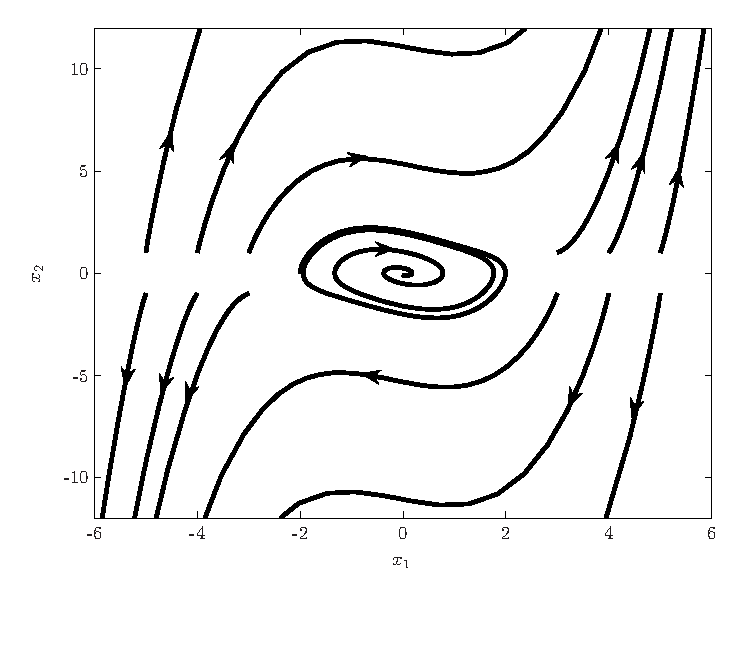
\includegraphics{images/OpenTraj.pdf}}}
\centerline{Trajectories of the open loop system}  
}

  \frame
  {
    \frametitle{Extension of linear controllers to PWA controllers}
\centerline{\resizebox{9cm}{!}{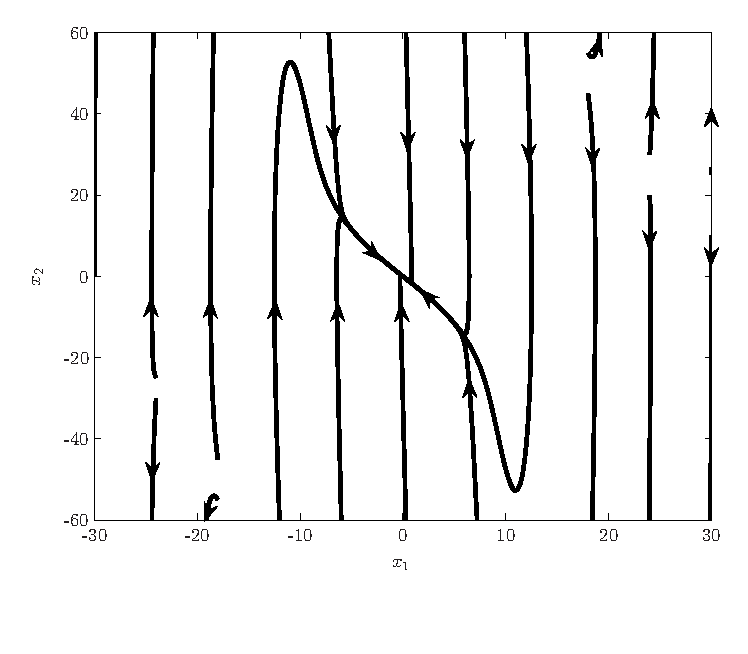
\includegraphics{images/LinTraj.pdf}}}
\centerline{Trajectories of the closed-loop system for the linear controller}
}

  \frame
  {
    \frametitle{Extension of linear controllers to PWA controllers}
\centerline{\resizebox{9cm}{!}{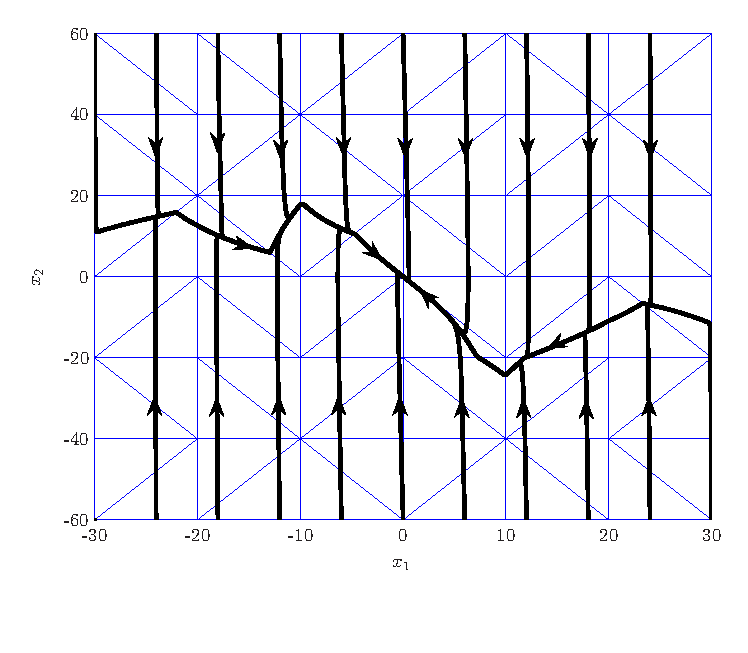
\includegraphics{images/PWATraj.pdf}}}
\centerline{Trajectories of the closed-loop system for the PWA controller}
}
  
  \frame
  {
    \frametitle{Extension of linear controllers to PWA controllers}
    \begin{itemize}
    \item \emph{The main limitation:} The controller synthesis is formulated as a set of Bilinear Matrix Inequalities (BMI). 
    \item \emph{Linear systems analogy:} Consider the linear system $\dot x = Ax+Bu$ with a candidate Lyapunov function $V(x)=x^\TR {\red P}x$ and a state feedback controller $u={\red K}x$. Sufficient conditions for the stability of this system are: 
    \begin{itemize}
    \item Positivity: $V(x)=x^\TR{\red P}x>0$ for $x\neq 0$ 
    \item Monotonicity: $\dot V(x)=\dot x^\TR{\red P}x+ x^\TR{\red P}\dot x<0$
    \end{itemize}
    \begin{align}
    &{\red P}>0\nonumber\\
    &(A^\TR+{\red K}^\TR B^\TR) {\red P}+{\red P}(A+B{\red K})<0\nonumber
    \end{align}
    \item BMIs are nonconvex problems in general.
    \end{itemize}
}

 \frame
  {
    \frametitle{Extension of linear controllers to PWA controllers}
    Contributions:
    \begin{itemize}
    \item To propose a two-step controller synthesis method for a class of uncertain nonlinear systems described by PWA differential inclusions.
    \begin{itemize}
    \item The proposed method has two objectives: global stability and local performance. It thus enables to use well known techniques in linear control design for local stability and performance while delivering a global PWA controller that is guaranteed to stabilize the nonlinear system.
    \item Differential inclusions are considered. Therefore the controller is robust in the sense that it can stabilize any piecewise smooth nonlinear system bounded by the differential inclusion.
    \item Stability is guaranteed even if sliding modes exist.
    \end{itemize}
    \end{itemize}
}  

%%%%%%%%%%%%%%%%%%%%%%%%%%%%%%%%%%%%%%%%%%%%%%%%%%%%%%%%%%%%%%%%%%%%%%%%%%%%%%%%%%%


  \section[]{Controller synthesis for PWA slab differential inclusions}
  \frame
  {
    \frametitle{A duality-based convex optimization approach}
\emph{Linear systems analogy:}
\begin{itemize}
    \item Consider the dual system 
    \beq
    \dot z=(A+B{\red K})^\TR z
    \eeq 
    with a candidate Lyapunov function 
    \beq
    V(x)=x^\TR {\red Q}x
    \eeq 
    \item Sufficient conditions for the stability of this system are: 
    \begin{itemize}
    \item Positive definiteness: ${\red Q}>0$
    \item Monotonicity: $(A+B{\red K}) {\red Q}+{\red Q}(A^\TR+{\red K}^\TR B^\TR)<0$
    \end{itemize}
    Define ${\red Y}={\red KQ}$.
    \begin{itemize}
    \item Positive definiteness: ${\red Q}>0$
    \item Monotonicity: $A{\red Q}+B{\red Y} +{\red Q}A^\TR+{\red Y}^\TR B^\TR<0$
    \end{itemize}
    Then ${\red K}={\red YQ^{-1}}$.
    \end{itemize}
  }
  
    \frame
  {
    \frametitle{A duality-based convex optimization approach}
    \begin{itemize}
    \item PWA slab system:
\begin{align}
\dot x =&A_{i}x+a_{i},\ x\in{\mathcal R}_i\nonumber\\
{\mathcal R}_i=& \{x|\ \|L_ix+l_i\|<1 \}\nonumber
\end{align}
\item Literature
\begin{itemize}
\item Hassibi and Boyd (1998)
\item Rodrigues and Boyd (2005)
\end{itemize}
\end{itemize}
  }

  \frame
  {
    \frametitle{A duality-based convex optimization approach}
    \begin{itemize}
\item Sufficient conditions for stability
\beq
P>0,
\eeq
\beq
A^\TR_{i}P+PA_{i}+\alpha P<0,\ \text{ for } 0\in \overline\RR_i,
\eeq
\beq
\left\{\begin{array}{c}
\lambda_{i}< 0,\\
	\left[\begin{matrix}
A^\TR_{i}P+PA_{i}+\alpha P+\lambda_{i}L_{i}^\TR L_{i}&Pa_{i}+\lambda_{i}l_{i}L_{i}^\TR \\
	a_{i}^\TR P+\lambda_{i}l_{i} L_{i}&\lambda_{i}(l_{i}^2-1)\\
	\end{matrix}\right]< 0, \text{ for } 0\notin \overline\RR_i
\end{array}\right.
\eeq
\item {Hassibi and Boyd (1998)}
\end{itemize}
}
  \frame
  {
    \frametitle{A duality-based convex optimization approach}
    \begin{itemize}
\item Sufficient conditions for stability
\beq
Q>0,
\eeq
\beq
A_{i}Q+QA^\TR_{i}+\alpha Q<0,\  \text{ for } 0\in \overline\RR_i,
\eeq
\beq
\left\{\begin{array}{c}
\mu_{i}< 0,\\
	\left[\begin{matrix}
A_{i}Q+QA^\TR_{i}+\alpha Q+\mu_{i}a_{i} a_{i}^\TR&QL_{i}^\TR+\mu_{i}l_{i}a_{i}\\
	L_{i}Q+\mu_{i}l_{i} a_{i}^\TR&\mu_{i}(l_{i}^2-1)\\
	\end{matrix}\right]< 0,\text{ for } 0\notin \overline\RR_i
	\end{array}\right. 
\eeq
\item {Hassibi and Boyd (1998)}
\end{itemize}
}

  \frame
  {
    \frametitle{A duality-based convex optimization approach}
    \begin{itemize}
    \item Parameter set:
\beq
\Omega =\left\{ \left.\bmat{cc}A_{i}&a_{i}\\L_i&l_i\emat\ \right| i=1,\ldots,M \right\}
\eeq
\item Dual parameter set
\beq
\Omega^\TR =\left\{ \left.\bmat{cc}A_{i}^\TR&L_i^\TR\\a_{i}^\TR&l_i\emat\ \right|\ i=1,\ldots,M\right\}
\eeq
\end{itemize}
}

\frame
  {
    \frametitle{A duality-based convex optimization approach}
    \begin{itemize}
    \item PWA slab system:
\begin{align}
\dot x =& A_{i}x+a_{i}+B_{w_{i}}w, \nonumber\\
x\in&{\mathcal R}_i=\{x |\ \|L_ix+l_i\|<1\}, \nonumber\\
y =& C_{i}x+D_{w_{i}}w, \nonumber
\end{align}
\item Parameter set:
\beq
\Phi =\left\{ \left.\bmat{ccc}A_{i}&a_{i}&B_{w_{i}}\\
L_i&l_i&0\\C_{i}&0&D_{w_{i}}\ \emat\right|\ i=1,\ldots,M \right\}
\eeq
\item {Hassibi and Boyd (1998)}
\end{itemize}
 }

\frame
  {
    \frametitle{A duality-based convex optimization approach}
    Summary:
    \begin{itemize}
    \item Introducing PWA slab differential inclusions
    \item Introducing the dual parameter set
    \item Extending the L$_2$ gain analysis and synthesis to PWA slab differential inclusions with PWA outputs
    \item Extending the definition of the regions of a PWA slab differential inclusion
    \item Proposing two methods to formulate the PWA controller synthesis for PWA slab differential inclusions as a convex problem
    \end{itemize}
}  

%%%%%%%%%%%%%%%%%%%%%%%%%%%%%%%%%%%%%%%%%%%%%%%%%%%%%%%%%%%%%%%%%%%%%%%%%%%%%%%%%%%%
  \section[]{Backstepping Controller Synthesis for PWP Systems}

  \frame
  {
    \frametitle{Sum of Squares Programming}
A sum of squares program is a convex optimization program of the following form:
\begin{eqnarray*}
\text{Minimize}&&\sum_{j=1}^Jw_j\alpha_j\\
\text{subject to}&&f_{i,0}+\sum_{j=1}^J\alpha_jf_{i,j}(x) \text{ is SOS, for }i=1,\ldots,I
\end{eqnarray*}
where the $\alpha_j$'s are the scalar real decision variables, the $w_j$'s are some given real numbers, and the $f_{i,j}$ are some given multivariate polynomials.
\begin{itemize}
\item<2-> SOSTOOLS, a MATLAB toolbox that handles the general SOS programming, was developed by S. Prajna, A. Papachristodoulou and P. Parrilo. 
%\item P. A. Parrilo (2000), Structured Semidefinite Programs and Semialgebraic Geometry Methods in Robustness and Optimization, PhD thesis.
\end{itemize}    
}
\frame
  {
    \frametitle{Backstepping Controller Synthesis for PWP Systems: A Sum of Squares Approach}
\begin{itemize}
\item Consider the following PWP system:
\begin{align*}
\dot x =& f_i(x)+g_i(x)z,\ x\in\PR_i\\
\dot z =&u
\end{align*}
where
\beq
\PR_i = \{ x| E_i(x) \succ 0\}
\eeq
where $E_i(x)\in\RE^{p_i}$ is a vector polynomial function of $x$ and $\succ$ represents an elementwise inequality.
\end{itemize}
}

\frame
  {
    \frametitle{Backstepping Controller Synthesis for PWP Systems: A Sum of Squares Approach}
\textbf{Backstepping as a Lyapunov function construction method:}
\begin{itemize}
\item<1-> Consider $\dot x = f_i(x)+g_i(x)z,\ x\in\PR_i$
\item<2-> Assume that there exists a polynomial control $z=\gamma(x)$ and $V(x)$ is an SOS Lyapunov function for the closed loop system verifying
\beq
\left\{\begin{array}{l}V(x)-\lambda(x)\text{\ is SOS}\\
-\nabla V(x)^\TR(f_i(x)+g_i(x)\gamma(x))-\Gamma_i(x)^\TR E_i(x)-\alpha V(x)\text{\ is SOS}\end{array}\right.
\eeq
for $i=1,\ldots,M$ and any $\alpha>0$, where $\lambda(x)$ is a positive definite SOS polynomial, $\Gamma_i(x)$ is an SOS vector function
\item<3-> Consider now the following candidate Lyapunov function 
\beq
V_\gamma(x,z)=V(x)+\frac{1}{2}(z-\gamma(x))^\TR (z-\gamma(x))
\eeq
Note that $V_\gamma(x,z)$ is a positive definite function. 
\end{itemize}
}

\frame
  {
    \frametitle{Backstepping Controller Synthesis for PWP Systems: A Sum of Squares Approach}
\begin{itemize}
\item \emph{Controller synthesis}: The synthesis problem can be formulated as the following SOS program.
\begin{eqnarray*}
\text{Find }&&u=\gamma_2(x,z)\text{ and } \Gamma(x,z)\\
\text{s.t.}&&-\nabla_{x} V_{\gamma}(x,z)^\TR(f_{i}(x)+g_{i}(x)z)\\
&&-\nabla_{z} V_{\gamma}(x,z)^\TR u\nonumber\\
&&-\Gamma(x,z)^\TR E_{i}(x,z)-\alpha V_\gamma(x,z)\text{\ is SOS},\nonumber\\
&&\Gamma(x,z)\text{\ is SOS}\nonumber\\
&&\gamma_2(0,0)=0
\end{eqnarray*}
where $i_2=1,\ldots,M_2$ and $\gamma_2(x_1,x_2)$ is a polynomial function of $x_1$ and $x_2$. 
\end{itemize}
}

\frame
  {
    \frametitle{Backstepping Controller Synthesis for PWP Systems: A Sum of Squares Approach}
Example: Single link flexible joint robot:
\centerline{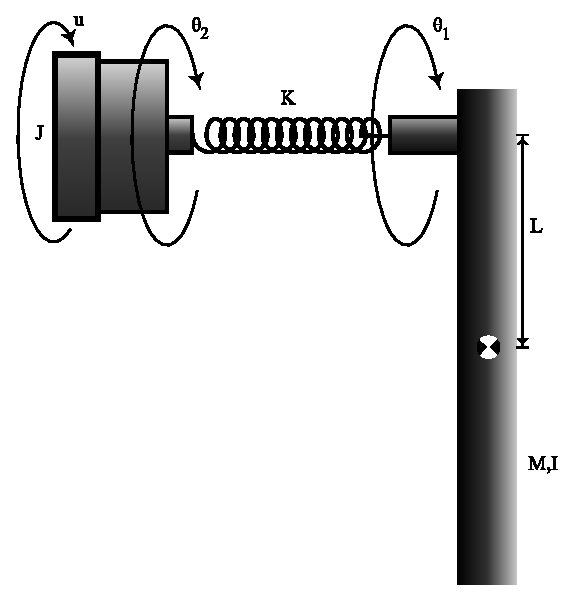
\includegraphics[width=6cm]{images/SLFJR.eps}}
}
\frame
  {
    \frametitle{Backstepping Controller Synthesis for PWP Systems: A Sum of Squares Approach}
Example: Single link flexible joint robot:
\begin{align*}
\dot x_1& = x_2\\
\dot x_2& = -\frac{MgL}{I}\sin(x_1)-\frac{K}{I}(x_1-x_3)\\
\dot x_3& = x_4\\
\dot x_4& = -\frac{f_2(x_4)}{J}+\frac{K}{J}(x_1-x_3)+\frac{1}{J}u
\end{align*}
where $x_1=\theta_1$, $x_2=\dot\theta_1$, $x_3=\theta_2$ and $x_4=\dot \theta_2$. $u$ is the motor torque and $f_2(x_4)$ denotes the motor friction which is described by
\beq
f_2(x_4)=b_mx_4+\sign(x_4)\left(F_{cm}+(F_{sm}-F_{cm})\exp(-\frac{x_4^2}{c_m^2})\right)
\eeq
}

\frame
  {
    \frametitle{Backstepping Controller Synthesis for PWP Systems: A Sum of Squares Approach}
PWP approximation:
\centerline{\resizebox{5cm}{!}{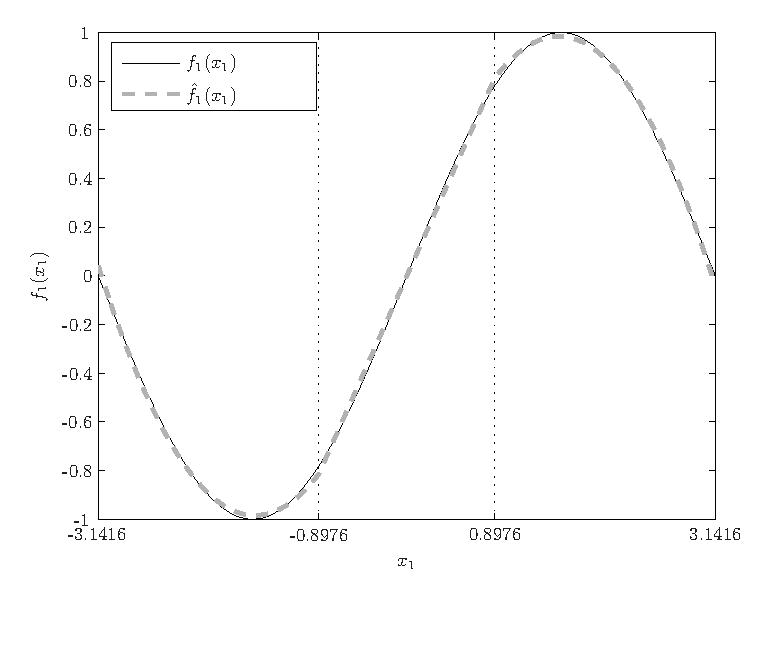
\includegraphics{images/f1app.pdf}}\resizebox{5cm}{!}{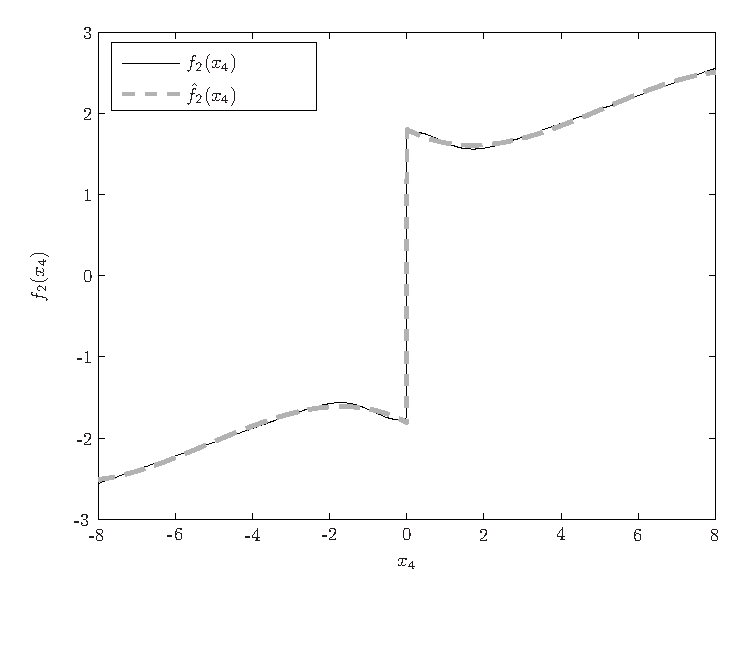
\includegraphics{images/f2app.pdf}}}
}
\frame
  {
    \frametitle{Backstepping Controller Synthesis for PWP Systems: A Sum of Squares Approach}
    \centerline{Typical structure of the regions of a PWP system in strict feedback form}
\centerline{\resizebox{10cm}{!}{
\xymatrix{
x_1& & & & \PR_{11}\ar[dll]\ar[d]\ar[drr] & & &\\
(x_1,x_2)& &\PR_{21}\ar[d]& &\PR_{22}\ar[d]& & \PR_{23}\ar[d]& \\
(x_1,x_2,x_3)&&\PR_{31}\ar[dl]\ar[d]& &\PR_{32}\ar[dl]\ar[dr]& & \PR_{33}\ar[d]\ar[dr]& \\
(x_1,x_2,x_3,x_4)&\PR_{41} &\PR_{44} & \PR_{42} & & \PR_{45} &\PR_{43} & \PR_{46} \\
}}}
}

\frame
  {
    \frametitle{Backstepping Controller Synthesis for PWP Systems: A Sum of Squares Approach}
State variables of the nonlinear model - PWA controller:
\centerline{\resizebox{8cm}{!}{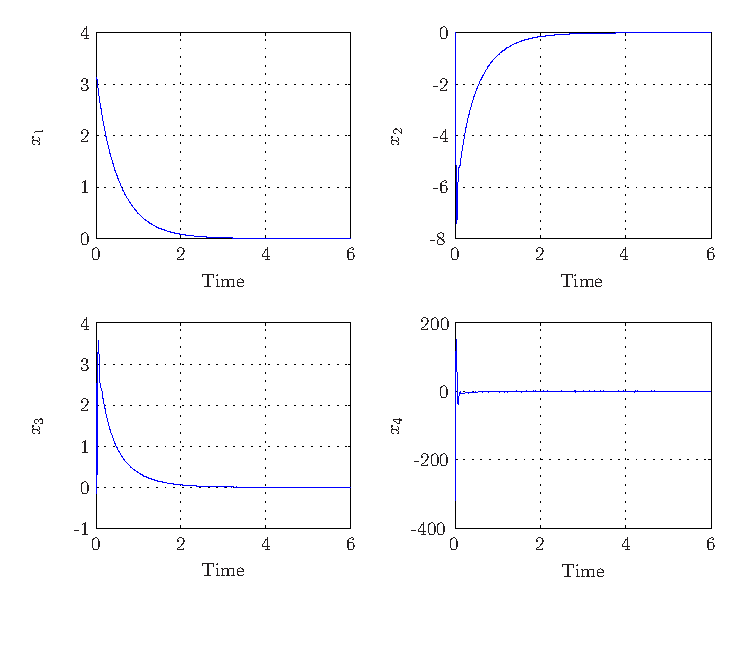
\includegraphics{images/stpwa.pdf}}}    
}

\frame
  {
    \frametitle{Backstepping Controller Synthesis for PWP Systems: A Sum of Squares Approach}
Control input - PWA controller:
\centerline{\resizebox{8cm}{!}{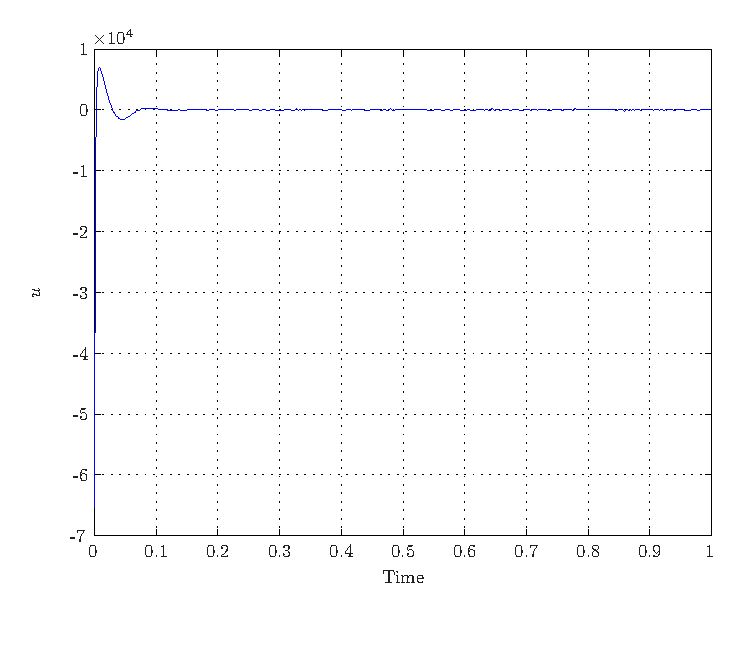
\includegraphics{images/inpwa.pdf}}}    
}

\frame
  {
    \frametitle{Backstepping Controller Synthesis for PWP Systems: A Sum of Squares Approach}
State variables of the nonlinear model - PWP controller:
\centerline{\resizebox{8cm}{!}{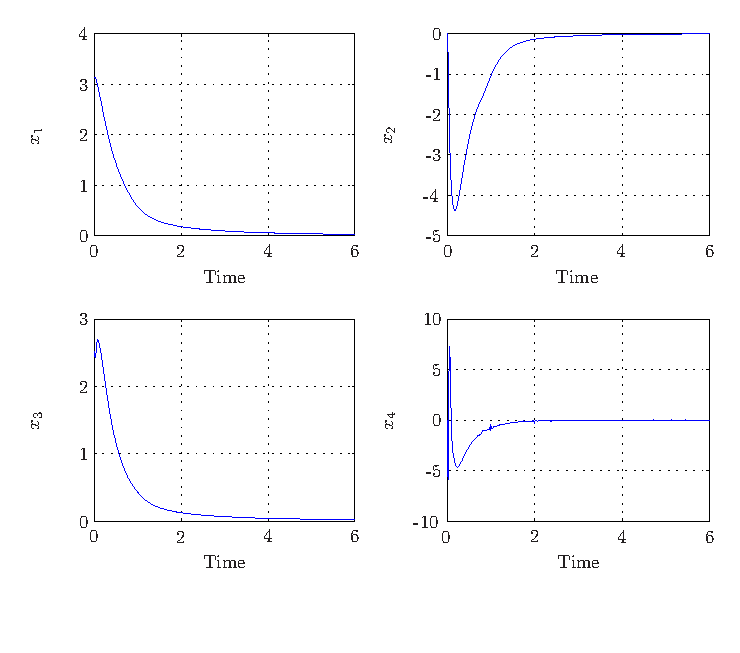
\includegraphics{images/stpwp.pdf}}}    
}

\frame
  {
    \frametitle{Backstepping Controller Synthesis for PWP Systems: A Sum of Squares Approach}
Control input - PWP controller:
\centerline{\resizebox{8cm}{!}{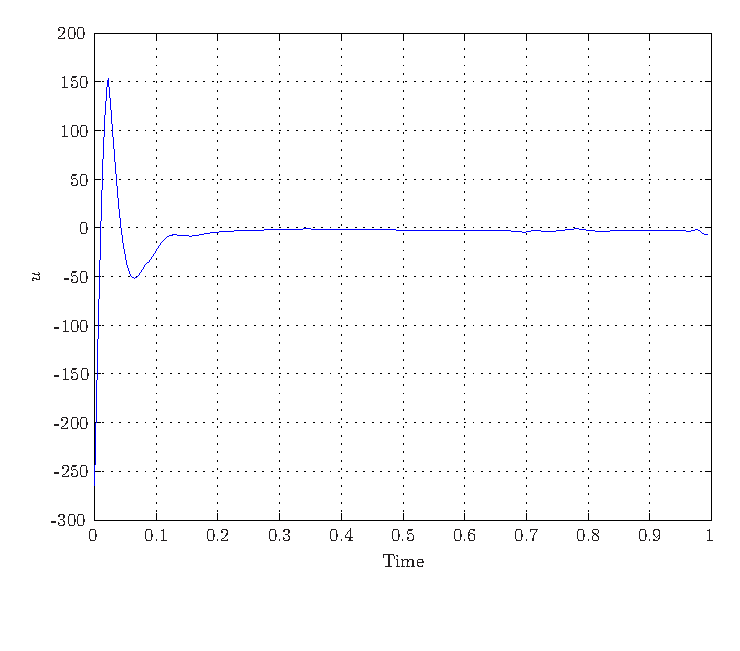
\includegraphics{images/inpwp.pdf}}}    
}
  
\frame
  {
    \frametitle{Backstepping Controller Synthesis for PWP Systems: A Sum of Squares Approach}
    Summary of the contributions:
    \begin{itemize}
    \item Introducing PWP systems in \emph{strict feedback form}
    \item Formulating backstepping controller synthesis for PWP systems as a convex optimization problem
    \begin{itemize}
    \item Polynomial Lyapunov functions for PWP systems with discontinuous vector fields
    \item PWP Lyapunov functions for PWP systems with continuous vector fields
    \item Numerical tools such as SOSTOOLS and Yalmip/SeDuMi
    \end{itemize}
		\end{itemize}
}  

\section[]{Sampled-Data PWA Systems}
  \frame
  {
    \frametitle{Sampled-Data PWA Systems: A Time-Delay Approach}
\begin{itemize}
\item<1-> PWA system
\beq
\dot x=A_ix+a_i+B_iu,\ \text{ for }x\in\RR_i
\eeq
with the region $\RR_i$ defined as
\beq
\RR_i=\{x| E_ix+e_i\succ 0\},
\eeq
\item<2-> Continuous-time PWA controller
\beq
u(t)=K_ix(t)+k_i,\ x(t)\in\RR_i
\eeq
\end{itemize}
}  

  \frame
  {
    \frametitle{Sampled-Data PWA Systems: A Time-Delay Approach}
    \begin{itemize}
    \item Lyapunov-Krasovskii functional:
\beq
V(x_s,\rho) := V_1(x)+V_2(x_s,\rho)+V_3(x_s,\rho)
\eeq
where 
\begin{eqnarray}
x_s(t) &:=& \bmat{c}x(t)\\x(t_k)\emat,\ t_k\leq t<t_{k+1}\nonumber
\end{eqnarray}
\begin{eqnarray}
V_1(x)&:=&x^\TR Px\nonumber\\
V_2(x_s,\rho)&:=&\int_{-\tau_M}^0\int_{t+r}^t\dot x^\TR(s)R\dot x(s)dsdr\nonumber\\
V_3(x_s,\rho)&:=&(\tau_M-\rho)(x(t)-x(t_k))^\TR X(x(t)-x(t_k))\nonumber
\end{eqnarray}
and $P$, $R$ and $X$ are positive definite matrices.
\end{itemize}
  }

  \frame
  {  
    \frametitle{Sampled-Data PWA Systems: A Time-Delay Approach}
\begin{itemize}
\item for all $i$ such that $0\in\overline\RR_i$,
{\scriptsize 
\beq
\bmat{cc}\Psi_i+\tau_M {M_1}_i&\bmat{c}P\\0\emat B_i+\tau_M\bmat{c}I\\-I\emat X B_i\\B_i^\TR\bmat{cc}P&0\emat+\tau_M B_i^\TR X\bmat{cc}I&-I\emat &-\gamma I\emat<0
\eeq
\beq
\bmat{ccc}\Psi_i+\tau_M {M_2}_i&\tau_M\bmat{c}A_i^\TR\\K_i^\TR B_i^\TR\emat R B_i+\bmat{c}P\\0\emat B_i&\tau_M N_i\\
\tau_M B_i^\TR R \bmat{cc} A_i & B_i K_i\emat+B_i^\TR\bmat{cc}P&0\emat&\tau_M B_i^\TR R B_i-\gamma I & 0\\
\tau_M N_i^\TR & 0 & -\frac{\tau_M}{2} R\emat<0
\eeq}
\end{itemize}
}

  \frame
  {  
    \frametitle{Sampled-Data PWA Systems: A Time-Delay Approach}
\begin{itemize}
\item for all $i$ such that $0\notin\overline\RR_i$, $\bar\Lambda_i\succ0$,
{\scriptsize 
\beq
\bmat{cc}\overline \Psi_i+\tau_M {\overline M_1}_i&\bmat{c}P\\0\\0\emat B_i+\tau_M\bmat{c}I\\-I\\0\emat X B_i\\B_i^\TR\bmat{ccc}P&0&0\emat+\tau_M B_i^\TR X\bmat{ccc}I&-I&0\emat&-\gamma I\emat<0
\eeq
\beq
\bmat{c|c|c}
\overline\Psi_i+\tau_M {\overline M_2}_i&\begin{array}{c}\tau_M\bmat{c}A_i^\TR\\K_i^\TR B_i^\TR\\k_i^\TR B_i^\TR +a_i^\TR\emat R B_i\\+\bmat{c}P\\0\\0\emat B_i\end{array}&\tau_M \bmat{c}N_i\\0\emat\\\noalign{\smallskip\hrule\smallskip}
\begin{array}{c}\tau_M B_i^\TR R \bmat{ccc} A_i & B_i K_i&B_i k_i+a_i \emat\\+B_i^\TR\bmat{ccc}P&0&0\emat\end{array} & \tau_M B_i^\TR R B_i-\gamma I & 0\\\noalign{\smallskip\hrule\smallskip}
\tau_M \bmat{cc}N_i^\TR&0\emat & 0 & -\frac{\tau_M}{2} R
\emat<0
\eeq}
\end{itemize}
}

  \frame
  {  
    \frametitle{Sampled-Data PWA Systems: A Time-Delay Approach}
	Summary of the contributions
    \begin{itemize}
    \item Formulating stability analysis of sampled-data PWA systems as a convex optimization problem
   \end{itemize}
  }

\section[]{Examples}
  \frame
  {
    \frametitle{Active Suspension System}
    Example: Active suspension with a nonlinear damper
    \centerline{\scalebox{0.3}{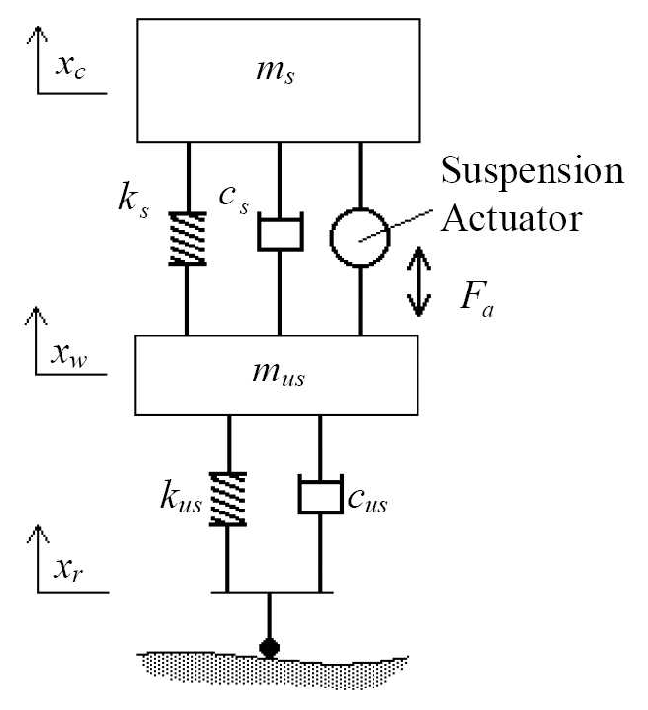
\includegraphics{images/ActiveSuspension.eps}\hspace{1cm} 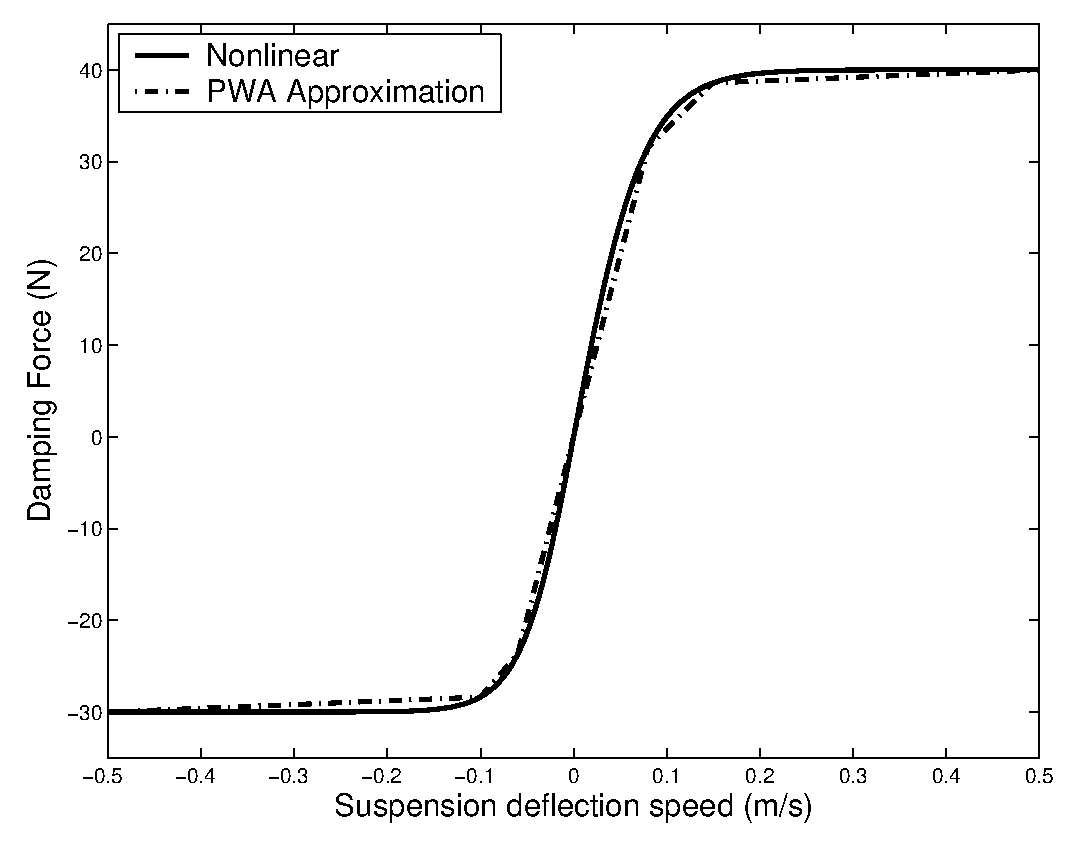
\includegraphics{images/pwapx.eps}}}
  }

\end{document}
